%  LaTeX support: latex@mdpi.com 
%  In case you need support, please attach all files that are necessary for compiling as well as the log file, and specify the details of your LaTeX setup (which operating system and LaTeX version / tools you are using).

%=================================================================
\documentclass[applsci,article,accept,moreauthors,pdftex]{Definitions/mdpi} 

% If you would like to post an early version of this manuscript as a preprint, you may use preprint as the journal and change 'submit' to 'accept'. The document class line would be, e.g., \documentclass[preprints,article,accept,moreauthors,pdftex]{mdpi}. This is especially recommended for submission to arXiv, where line numbers should be removed before posting. For preprints.org, the editorial staff will make this change immediately prior to posting.

%--------------------
% Class Options:
%--------------------
%----------
\usepackage{array}
% journal
%----------
% Choose between the following MDPI journals:
% acoustics, actuators, addictions, admsci, aerospace, agriculture, agriengineering, agronomy, algorithms, animals, antibiotics, antibodies, antioxidants, applsci, arts, asc, asi, atmosphere, atoms, axioms, batteries, bdcc, behavsci , beverages, bioengineering, biology, biomedicines, biomimetics, biomolecules, biosensors, brainsci , buildings, cancers, carbon , catalysts, cells, ceramics, challenges, chemengineering, chemistry, chemosensors, children, cleantechnol, climate, clockssleep, cmd, coatings, colloids, computation, computers, condensedmatter, cosmetics, cryptography, crystals, dairy, data, dentistry, designs , diagnostics, diseases, diversity, drones, econometrics, economies, education, ejihpe, electrochem, electronics, energies, entropy, environments, epigenomes, est, fermentation, fibers, fire, fishes, fluids, foods, forecasting, forests, fractalfract, futureinternet, futurephys, galaxies, games, gastrointestdisord, gels, genealogy, genes, geohazards, geosciences, geriatrics, hazardousmatters, healthcare, heritage, highthroughput, horticulturae, humanities, hydrology, ijerph, ijfs, ijgi, ijms, ijns, ijtpp, informatics, information, infrastructures, inorganics, insects, instruments, inventions, iot, j, jcdd, jcm, jcp, jcs, jdb, jfb, jfmk, jimaging, jintelligence, jlpea, jmmp, jmse, jnt, jof, joitmc, jpm, jrfm, jsan, land, languages, laws, life, literature, logistics, lubricants, machines, magnetochemistry, make, marinedrugs, materials, mathematics, mca, medicina, medicines, medsci, membranes, metabolites, metals, microarrays, micromachines, microorganisms, minerals, modelling, molbank, molecules, mps, mti, nanomaterials, ncrna, neuroglia, nitrogen, notspecified, nutrients, ohbm, optics, particles, pathogens, pharmaceuticals, pharmaceutics, pharmacy, philosophies, photonics, physics, plants, plasma, polymers, polysaccharides, preprints , proceedings, processes, proteomes, psych, publications, quantumrep, quaternary, qubs, reactions, recycling, religions, remotesensing, reports, resources, risks, robotics, safety, sci, scipharm, sensors, separations, sexes, signals, sinusitis, smartcities, sna, societies, socsci, soilsystems, sports, standards, stats, surfaces, surgeries, sustainability, symmetry, systems, technologies, test, toxics, toxins, tropicalmed, universe, urbansci, vaccines, vehicles, vetsci, vibration, viruses, vision, water, wem, wevj

%---------
% article
%---------
% The default type of manuscript is "article", but can be replaced by: 
% abstract, addendum, article, benchmark, book, bookreview, briefreport, casereport, changes, comment, commentary, communication, conceptpaper, conferenceproceedings, correction, conferencereport, expressionofconcern, extendedabstract, meetingreport, creative, datadescriptor, discussion, editorial, essay, erratum, hypothesis, interestingimages, letter, meetingreport, newbookreceived, obituary, opinion, projectreport, reply, retraction, review, perspective, protocol, shortnote, supfile, technicalnote, viewpoint
% supfile = supplementary materials

%----------
% submit
%----------
% The class option "submit" will be changed to "accept" by the Editorial Office when the paper is accepted. This will only make changes to the frontpage (e.g., the logo of the journal will get visible), the headings, and the copyright information. Also, line numbering will be removed. Journal info and pagination for accepted papers will also be assigned by the Editorial Office.

%------------------
% moreauthors
%------------------
% If there is only one author the class option oneauthor should be used. Otherwise use the class option moreauthors.

%---------
% pdftex
%---------
% The option pdftex is for use with pdfLaTeX. If eps figures are used, remove the option pdftex and use LaTeX and dvi2pdf.

%=================================================================
\firstpage{1} 
\makeatletter 
\setcounter{page}{\@firstpage} 
\makeatother
\pubvolume{xx}
\issuenum{1}
\articlenumber{5}
\pubyear{2020}
\copyrightyear{2020}
%\externaleditor{Academic Editor: name}
\history{Received: date; Accepted: date; Published: date}
\updates{yes} % If there is an update available, un-comment this line

%% MDPI internal command: uncomment if new journal that already uses continuous page numbers 
%\continuouspages{yes}

%------------------------------------------------------------------
% The following line should be uncommented if the LaTeX file is uploaded to arXiv.org
%\pdfoutput=1
\usepackage{booktabs} 
\usepackage{multirow}
\usepackage{soul}
\usepackage{microtype}
\usepackage{upgreek}
\setitemize{parsep=6pt,itemsep=0pt,leftmargin=*,labelsep=5.8mm,align=parleft}  
\setenumerate{parsep=6pt,itemsep=0pt,leftmargin=*,labelsep=4.9mm,align=parleft}  
\setlist[description]{itemsep=0mm}

\usepackage{hyperref}
%\makeatletter
%\g@addto@macro{\UrlBreaks}{\UrlOrds}
%\makeatother
\makeatletter
\def\UrlAlphabet{%
\do\a\do\b\do\c\do\d\do\e\do\f\do\g\do\h\do\i\do\j%
\do\k\do\l\do\m\do\n\do\o\do\p\do\q\do\r\do\s\do\t%
\do\u\do\v\do\w\do\x\do\y\do\z\do\A\do\B\do\C\do\D%
\do\E\do\F\do\G\do\H\do\I\do\J\do\K\do\L\do\M\do\N%
\do\O\do\P\do\Q\do\R\do\S\do\T\do\U\do\V\do\W\do\X%
\do\Y\do\Z}
\def\UrlDigits{\do\1\do\2\do\3\do\4\do\5\do\6\do\7\do\8\do\9\do\0}
\g@addto@macro{\UrlBreaks}{\UrlOrds}
\g@addto@macro{\UrlBreaks}{\UrlAlphabet}
\g@addto@macro{\UrlBreaks}{\UrlDigits}
\makeatother
%=================================================================
% Add packages and commands here. The following packages are loaded in our class file: fontenc, calc, indentfirst, fancyhdr, graphicx, lastpage, ifthen, lineno, float, amsmath, setspace, enumitem, mathpazo, booktabs, titlesec, etoolbox, amsthm, hyphenat, natbib, hyperref, footmisc, geometry, caption, url, mdframed, tabto, soul, multirow, microtype, tikz

\usepackage{rotating}
\usepackage{makecell}
\usepackage{changepage}
%\usepackage[landscape]{geometry}
\usepackage{pdflscape}
%=================================================================
%% Please use the following mathematics environments: Theorem, Lemma, Corollary, Proposition, Characterization, Property, Problem, Example, ExamplesandDefinitions, Hypothesis, Remark, Definition, Notation, Assumption
%% For proofs, please use the proof environment (the amsthm package is loaded by the MDPI class).

%=================================================================
% Full title of the paper (Capitalized)
\Title{Linked Data Platform for \textit{Solanaceae} Species} %Attention AE/ME. The following layout issues have not been checked by the English Editing Department and must be carefully verified by the AE/Layout Department: All callout issues, bold usage of callouts, and references to callouts in the text. Correct callout usage in figures. Figure and Table layout issues. Footnote formatting and Glossaries have not been checked. En dash usage for negative values, en dash usage to indicate relationships, en dash usage to indicate bonds (especially in chemistry). The English Editing Department is not responsible for correct italic usage for genes, proteins and technical terminology. This responsibility belongs to the authors. The following are also not checked: spacing between numbers and units of measurement, ratios, en dashes for ranges, date and time formats, punctuation in equation lines, and less than/more than spacing (< >). Finally, capitalization and layout of titles/headings must be properly checked as well as ensuring 'Eq.' and 'Fig.' are properly spelled out, as these are layout issues.

% Author Orchid ID: enter ID or remove command
\newcommand{\orcidauthorA}{0000-0003-1615-4197} % Add \orcidA{} behind the author's name
\newcommand{\orcidauthorB}{0000-0003-1711-7961} % Add \orcidB{} behind the author's name

\newcommand{\orcidauthorC}{0000-0001-8183-0484} % Add \orcidB{} behind the author's name

\newcommand{\orcidauthorD}{0000-0002-4368-8058} % Add \orcidB{} behind the author's name

\newcommand{\orcidauthorE}{0000-0001-5565-7577} % Add \orcidE{} behind the author's name
\newcommand{\orcidauthorF}{0000-0002-0213-4016} % Add \orcidE{} behind the author's name

\newcommand{\orcidauthorG}{0000-0002-3077-6833} % Add \orcidG{} behind the author's name
\newcommand{\orcidauthorH}{0000-0001-5417-5066} % Add \orcidH{} behind the author's name

% Authors, for the paper (add full first names)
%\Author{Firstname Lastname $^{1,\dagger,\ddagger}$\orcidA{}, Firstname Lastname $^{1,\ddagger}$ and Firstname Lastname $^{2,}$*}
\Author{\hl{Gurnoor Singh} %MDPI: Please carefully check the accuracy of names and affiliations.
 $^{1,\dagger,\ddagger}$\orcidA{}, Arnold Kuzniar $^{2,}$*$^{,\ddagger}$\orcidB{}, Matthijs Brouwer $^{1}$\orcidC{}, Carlos Martinez-Ortiz $^{2}$\orcidE{}, Christian W. B. Bachem $^{1}$\orcidG{}, \hl{Yury} %MDPI: it is different from redmine. This is correct
 M\hl{.} %MDPI: newly add. Ok
 Tikunov $^{1}$\orcidH{}, Arnaud G. Bovy $^{1}$, \hl{Richard G. F. Visser} %MDPI: its order is different from redmine and we add space between G. and F. OK
$^{1}$\orcidF{} and~Richard Finkers $^{1,}$*\orcidD{}}


% Authors, for metadata in PDF
\AuthorNames{Gurnoor Singh, Arnold Kuzniar, Matthijs Brouwer, Carlos Martinez-Ortiz, Christian W. B. Bachem, Yury M. Tikunov, Arnaud G. Bovy, Richard G. F. Visser and Richard Finkers}

% Affiliations / Addresses (Add [1] after \address if there is only one affiliation.)
\address{%
$^{1}$ \quad Plant Breeding, Wageningen University and Research,  \hl{6708 PB} %MDPI: newly add post code, same as below highlight. OK
Wageningen, The Netherlands; \hl{gurnoor1990@gmail.com (G.S.); matthijs.brouwer@wur.nl (M.B.); Christian.Bachem@wur.nl (C.W.B.B.); Yury.tikunov@wur.nl (Y.M.T.); arnaud.bovy@wur.nl (A.G.B.); richard.visser@wur.nl (R.G.F.V.)} %MDPI: Newly add. OK
 \\
$^{2}$ \quad Netherlands eScience Center, \hl{1098 XG} Amsterdam, The Netherlands; \hl{c.martinez@esciencecenter.nl}}

% Contact information of the corresponding author
\corres{Correspondence: \hl{a.kuzniar@esciencecenter.nl (A.K.); richard.finkers@wur.nl (R.F.)}}

% Current address and/or shared authorship
\firstnote{Current address: The Center for Molecular and Biomolecular Informatics (CMBI), Radboud University Medical Center, \hl{6525 GA}, Nijmegen, The Netherlands.}  %MDPI: Please add post code. Added
\secondnote{These authors contributed equally to this work.}
% The commands \thirdnote{} till \eighthnote{} are available for further notes

%\simplesumm{} % Simple summary

%\conference{} % An extended version of a conference paper

% Abstract (Do not insert blank lines, i.e.  \\) 
\abstract{Genetics research is increasingly focusing on mining fully sequenced genomes and their annotations to identify the causal genes associated with traits (phenotypes) of interest. However, a~complex trait is typically associated with multiple quantitative trait loci (QTLs), each~comprising many genes, that can positively or negatively affect the trait of interest. To help breeders in ranking candidate genes, we developed an analytical platform called pbg-ld that provides semantically integrated geno- and phenotypic data on \textit{Solanaceae}%italics added
	 species.~This platform combines both unstructured data from scientific literature and structured data from publicly available biological databases using the Linked Data approach. In particular, QTLs were extracted from tables of full-text articles from the Europe PMC %please define | this is reference 35, should it be here (QTM v1.1.0)
repository using QTLTableMiner\textsuperscript{++}, while the genomic annotations were obtained from the Sol Genomics Network (SGN), UniProt, and Ensembl Plants databases. These~datasets were transformed into Linked Data graphs, which include cross-references to many other relevant databases such as Gramene, Plant Reactome, InterPro and KEGG Orthology (KO), and so forth. Users~can query and analyze the integrated data through a web interface or programmatically via the SPARQL and RESTful services (APIs). We illustrate the usability of pbg-ld with the help of querying the genome annotations, comparing genome graphs, and two biological use cases. In the biological use case 1 we illustrate a comparative genomics study using pbg-ld to compare the difference in the genetic mechanism underlying tomato fruit shape and potato tuber-shape. In biological use case 2, %comma added
 we illustrate the usability of pbg-ld in developing a seamlessly integrative workflow that uses genomic data from pbg-ld knowledge graphs and prioritization pipelines to predict candidate genes within QTL regions for metabolic traits of tomato.
}


% Keywords
\keyword{{prioritization of candidate genes; plant breeding; \textit{Solanaceae}; QTLs; semantic web; linked~data}}

% The fields PACS, MSC, and JEL may be left empty or commented out if not applicable
%\PACS{J0101}
%\MSC{}
%\JEL{}

%%%%%%%%%%%%%%%%%%%%%%%%%%%%%%%%%%%%%%%%%%
% Only for the journal Diversity
\LSID{\textbf{\hl{Source code and availability}:} \url{https://github.com/candYgene/pbg-ld}}%MDPI: Please check if this can be removed to back matter part or main text?  No, we consider this to be central for the paper and would like to see this emphasized here.

%%%%%%%%%%%%%%%%%%%%%%%%%%%%%%%%%%%%%%%%%%
% Only for the journal Applied Sciences:
%\featuredapplication{Authors are encouraged to provide a concise description of the specific application or a potential application of the work. This section is not mandatory.}
%%%%%%%%%%%%%%%%%%%%%%%%%%%%%%%%%%%%%%%%%%

%%%%%%%%%%%%%%%%%%%%%%%%%%%%%%%%%%%%%%%%%%
% Only for the journal Data:
%\dataset{DOI number or link to the deposited data set in cases where the data set is published or set to be published separately. If the data set is submitted and will be published as a supplement to this paper in the journal Data, this field will be filled by the editors of the journal. In this case, please make sure to submit the data set as a supplement when entering your manuscript into our manuscript editorial system.}

%\datasetlicense{license under which the data set is made available (CC0, CC-BY, CC-BY-SA, CC-BY-NC, etc.)}

%%%%%%%%%%%%%%%%%%%%%%%%%%%%%%%%%%%%%%%%%%
% Only for the journal Toxins
%\keycontribution{The breakthroughs or highlights of the manuscript. Authors can write one or two sentences to describe the most important part of the paper.}

%\setcounter{secnumdepth}{4}
%%%%%%%%%%%%%%%%%%%%%%%%%%%%%%%%%%%%%%%%%%
\begin{document}
%%%%%%%%%%%%%%%%%%%%%%%%%%%%%%%%%%%%%%%%%%

%%%%%%%%%%%%%%%%%%%%%%%%%%%%%%%%%%%%%%%%%%
%\setcounter{section}{-1} %% Remove this when starting to work on the template.
%\section{How to Use this Template}
%The template details the sections that can be used in a manuscript. Note that the order and names of article sections may differ from the requirements of the journal (e.g., the positioning of the Materials and Methods section). Please check the instructions for authors page of the journal to verify the correct order and names. For any questions, please contact the editorial office of the journal or support@mdpi.com. For LaTeX related questions please contact latex@mdpi.com.
%The order of the section titles is: Introduction, Materials and Methods, Results, Discussion, Conclusions for these journals: aerospace,algorithms,antibodies,antioxidants,atmosphere,axioms,biomedicines,carbon,crystals,designs,diagnostics,environments,fermentation,fluids,forests,fractalfract,informatics,information,inventions,jfmk,jrfm,lubricants,neonatalscreening,neuroglia,particles,pharmaceutics,polymers,processes,technologies,viruses,vision

%%%%%%%%%%%%%%%%%%%%%%%%%%%%%%%%%%%%%%%%%%
\section{Introduction}
The availability of annotated reference genome assemblies for several crop species including tomato~\cite{tomato2012tomato}, potato~\cite{potato2011genome}, brassica~\cite{wang2011genome} and cucumber~\cite{huang2009genome} has enabled plant breeders and researchers to elucidate a trait’s linkage to a genomic location(s). Mining genome annotations can help in identifying candidate genes that positively or negatively affect a trait of interest, which plant breeders aim to improve. However, genome annotations are commonly available across multiple databases and file formats (e.g., in~the Generic Feature Format [GFF]), which hampers integrated data~analyses.

Traditionally, plant breeders identified chromosomal regions using genetic markers that are statistically associated with traits of interest. These genomic regions are called quantitative trait loci (QTLs). A~QTL region can easily contain thousands of genes including those that negatively influence the trait of interest~\cite{chibon2012marker2sequence}. Therefore, detecting the causative gene for breeding is of major importance. There are three major approaches to address the challenge of candidate gene prediction in crop species: (i) the analysis of gene expression data or co-expression networks~\cite{astola2014inferring}, (ii) comparative genomics~\cite{shinozuka2012quantitative}, and~(iii) integrate information stored in scientific literature and in molecular biology databases such as the ELIXIR Core Data Resources~\cite{durinx2016identifying} (including ENA %please define
~\cite{harrison2018european}, Ensembl Plants~\cite{bolser2017ensembl} and UniProt~\cite{pundir2017uniprot}) and the Sol Genomics Network (SGN) \cite{mueller2005sol}. To~address the need for improved access to integrated plant data, we developed the Solanaceae Linked Data platform (pbg-ld) \cite{Kuzniarpbgld} that combines QTLs from scientific literature and genome annotations from public databases using the Linked Data approach~\cite{Berners-Lee2006}. Our~approach is to create a semantic web of data rather than that of hypertext (HTML) documents using Uniform Resource Identifiers (URIs) and Resource Description Framework (RDF) [15]. A~URI is an HTTP-based resource identifier assigned to an entity whereas RDF is a generic graph-based data model for describing entities and their relationships. In~addition, publishing data according to FAIR Data Principles~\cite{wilkinson2016fair} further increases the degree of discoverability and (re-)usability of research~data.

In plant sciences, several controlled vocabularies and ontologies have been developed to standardize domain-specific terms and/or represent the current knowledge of the domain in a machine-readable form.~For~example, the~\textit{Solanaceae} %italics added
Phenotype Ontology (SPTO) \cite{SPTO}, Crop~Ontology~\cite{CO}, Plant Ontology (PO) \cite{doi:10.1093/pcp/pcs163}, Phenotypic Quality Ontology (PATO) \cite{Walls2012} and Trait Ontology (TO) \cite{TO} are used to identify plant-specific phenotypic information while Gene Ontology (GO) \cite{GOontology}, Sequence Ontology (SO) \cite{Eilbeck2005} and FALDO~\cite{FALDO} are used to identify genotypic information. Similarly, the~Chemical Entities of Biological Interest database/ontology (ChEBI) \cite{Hastings2013} is focused on small chemical~compounds. 

There are several plant-specific databases available that provide geno- and phenotypic%hyphen removed
 data. For~example, Ensembl Plants is a widely used integrated resource on plant genomes. Similarly, UniProt is a database of protein sequences, function annotations and proteomes of various species including plants. Both databases release their data in RDF-based format. The~\textit{Arabidopsis}%italixs added
  Information Resource (TAIR) \cite{garcia2002tair} is a resource to analyze and to compare molecular, biological, and~genetical data of the model species \textit{Arabidopsis thaliana}.%Italtics added on species name
 	 Further, the~Sol Genomics Network (SGN) \cite{mueller2005sol} provides genomic, genetic and phenotypic information for members of the \textit{Solanaceae}%italics added
 	  family. Plant Genome DataBase Japan (PGDBj) \cite{nakaya2017plant} is an integrated web resource for plant genome-related information from literature and public databases. However, the~TAIR, SGN, and~PGDBj do not distribute their data in a semantically interoperable (RDF) format. The~Planteome~\cite{Cooper2018} database provides gene annotations and phenotypes with the help of reference ontologies such as PO, TO, GO and ChEBI. Planteome is a user-friendly tool to query traits of interest, germplasm, and~putative candidate genes. However, it~lacks QTLs, genetic markers and links to publicly available databases such as Ensembl~Plants.

We present the pbg-ld platform that provides semantically integrated geno-/pheno-typic data on \textit{Solanaceae}%italics added 
species such as the (wild) tomato and potato species~\cite{kuzniar_arnold_2018_1458169}. The~resulting (linked) datasets are made available through a web interface or programmatic services (SPARQL and RESTful APIs). The~use of these data access points is described in the results section. Pbg-ld is an integrated plant resource that aids breeders in detecting candidate genes for complex traits using the knowledge available in the scientific literature and in public~databases.

%%%%%%%%%%%%%%%%%%%%%%%%%%%%%%%%%%%%%%%%%%

\section{Data Generation and Ingestion~Pipeline}

{{{All data sets used in the creation of this linked data platform were initially classified as non-RDF based and RDF based data sources. The~first step in our data ingestion pipeline was to convert non-RDF based data sources to RDF based data graphs. Later these RDF data graphs were integrated together and published as a linked data platform.}} Figure~\ref{Figure1} illustrates the data generation and ingestion pipeline used by the pbg-ld platform. Geno- and pheno-typic data from three \textit{Solanaceae}%itelics added
	 species:%colon added and dashes removed 
	 (i) reference sequence tomato (\textit{S. lycopersicum}), (ii) wild tomato (\textit{S. pennellii}) and (iii) the reference sequence potato  (\textit{S. tuberosum}) is collected and integrated into this~pipeline. 

\begin{figure}[H]
\centering
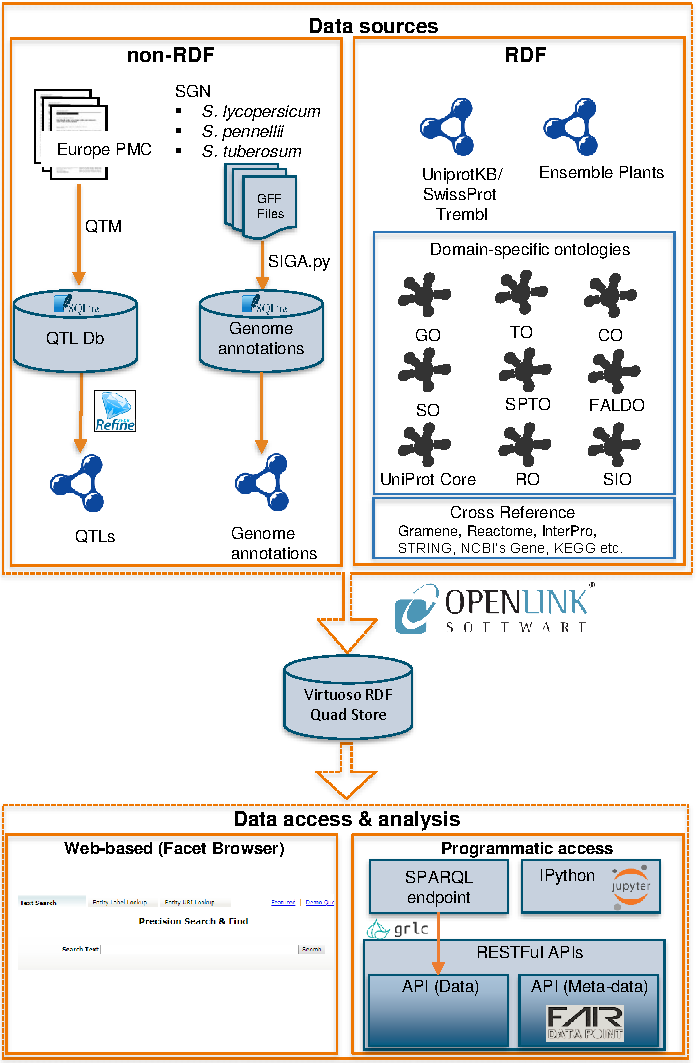
\includegraphics[scale=.95]{Figure1.pdf}
\caption{Data generation and ingestion pipeline. All data originate from either non-Resource Description Framework (RDF) or RDF sources. Several tools are used to retrieve and transform non-RDF data into RDF graphs: QTM %please define
is used to extract tomato and potato quantitative trait loci (QTLs) from Europe PMC %please define
 articles; OpenRefine is used to transform the QTLs into RDF according to the specified data model. Similarly, SIGA.py tool converts the genome annotations, as~provided by the Sol Genomics Network (SGN) in GFF files into RDF graphs with gene models and markers. In~addition, the~UniProt (proteomes) and Ensembl Plants (gene models) distribute their data in RDF format. All RDF graphs including domain-specific ontologies (in OWL) and database cross-references were stored and integrated with Virtuoso RDF Quad Store. The~resulting linked datasets are made available for queries and analyses through data-access layer: (i) Linked data browser, (ii) SPARQL endpoint, (iii) grlc-based Web API~\cite{Merono-Penuela2016} and (iv) FAIR Data Point (FDP) metadata (RESTful) service.}
\label{Figure1}
\end{figure}
\unskip


\subsection{Data Sources } 

To facilitate the integration of geno- and pheno-typic data of \textit{Solanaceae} %itelics added
species, we used data from (semi-)structured resources. Semi-structured data resources include scientific articles in XML file format obtained from Europe PMC or the General Feature Format(GFF)-based text file~\cite{europe2015europe,GFF3}. Moreover, semi-structured data were classified as non-RDF data and were subsequently transformed into (structured) RDF data. On~the contrary, structured data resources contained data in the form of RDF structure, for~example, genome annotation in Ensemble Plants and Uniprot, as~well as domain~ontologies.  

\subsubsection{QTL}
QTL studies have widely been published in scientific articles, particularly in tables or supplementary materials. However, there is no established repository where experimental data on plant-specific QTL studies can be submitted. Therefore, QTL information is extracted from XML based scientific literature and processed to RDF graphs using the QTL TableMiner\textsuperscript{++} (QTM) tool~\cite{singh2018qtltableminer++} version (v1.1.0) \cite{singh_gurnoor_2019_1193640}. QTM extracted 324 QTLs from a total of 21 \textit{Solanaceae}–specific full-text articles in the Europe PMC repository. 234 of these QTLs (i.e., 93 in tomato and 64 in potato) were associated with exact chromosomal locations based on flanking markers while the remaining 90 QTLs were associated with peak markers and/or candidate~genes. 

\subsubsection{SGN }
SGN provides genome annotations in GFF files for \textit{Solanaceae} %itelics added
species. The~GFF files were transformed into RDF graphs using the SIGA.py command-line tool (v0.5.1) \cite{Kuzniar2017} (\hl Figure \ref{FigureA1}). %MDPI: pleae check if here should be Appendix A1 Figure A1 here, and there is no this figure in the tex zip, please add it. This is now fixed
 The~gene models and the genetic markers of (wild) tomato (\textit{S. lycopersicum} and \textit{S. pennellii}) and potato (\textit{S. tuberosum}) were downloaded from the SGN’s FTP server (\url{ftp://ftp.solgenomics.net/genomes/}). For~\textit{S. lycopersicum}, the~genome annotations comprising of gene models, SGN markers, SolCAP markers, were taken from GFF files of the ITAG 2.4 released on 23-02-2014~\cite{LyocITAG2.4}. For~\textit{S.~pennelli}, the~genome annotations comprising of gene models (spenn{\_}v2.0) released on 27-08-2014, and~SGN markers released on 10-08-2014 were taken as input~\cite{PennITAG2.4}. Similarly, for~\textit{S. tuberosum}, genome annotations of PGSC{\_}DM (diploid/double monoploid) version 4.03 released on 04-09-2013 were used~\cite{PGSCDM}.

\subsubsection{Ensembl Plants and UniProt}
Ensembl Plants is an genome-centeric integrated resource for plant sciences. Genome annotations of \textit{S. lycopersicum} (release ITAG2.4 genome annotation based on SL2.50 genome assembly) \cite{EnsemblPlantSolanumlycopersicum} and \textit{S.~tuberosum} (release PGSC{\_}DM 3.0 genome annotation  based on SolTub3.0  genome assembly) were taken from the Ensembl Plants database (release 33) \cite{EnsemblPlantSolanumtuberosum} in RDF format. The~proteomes of \textit{S.~lycopersicum} \cite{UniprotSL} and \textit{S. tuberosum} \cite{UniprotST} were obtained from UniProt in the RDF/Turtle~format. 

\subsection{Ontologies}
Pbg-ld makes use of the following domain-specific ontologies: Gene Ontology (GO) \cite{GOontology}, \textit{Solanaceae} %itelics added
Phenotype Ontology (SPTO) \cite{SPTO}, Crop ontology (CO) \cite{CO}, Sequence Types and Features Ontology (SO) \cite{Eilbeck2005}, Feature Annotation Location Description Ontology (FALDO) \cite{FALDO}, Trait Ontology (TO) \cite{TO}, UniProt Core~\cite{UniprotRDFcore}, Semanticscience Integrated Ontology (SIO) \cite{SIO}, Relation Ontology (RO)~\cite{RO}, Plant Ontology (PO) \cite{doi:10.1093/pcp/pcs163}, Phenotypic Quality Ontology (PATO) \cite{Walls2012}.
\\\\


\subsection{Linked Data Deployment}
OpenLink’s Virtuoso Universal Server (version 7.20.3217, open-source edition) was used to store and connect the data graphs in the RDF Quad Store. Pbg-ld is made as a modular and re-deployable {software} with the help of Docker~\cite{boettiger2015introduction} and Ansible~\cite{ansible}. The~pbg-ld platform including the associated RESTful web services, namely the grlc-based API for data and the FAIR Data Point API for metadata, can be deployed locally by the~user.

%\cite{Faceted_Browser}
%\cite{Sparqlendpoint}
\subsection{Data Access \& Analysis}
Pbg-ld provides access to the (meta)data through a web-based user interface (Virtuoso Faceted Browser) and programmatic interfaces such as SPARQL and RESTful APIs.
Using the web-based user interface, a~user can query the RDF triples in three different ways through (i) a free-text search box, (ii)~an entity label search box or (iii) an entity URI search box. There is a SPARQL endpoint provided for a user to write and execute SPARQL queries on the RDF graphs available in the pbg-ld platform. Further, with~the help of grlc tool~\cite{Merono-Penuela2016}, we published customized RESTful APIs, built on the top of pbg-ld’s datasets to provide easy (programmatic) access based on the SPARQL endpoint. Data~consumers who do not know the SPARQL query language can use these APIs to query the platform. This way grlc hides the complexities or intricacies of SPARQL. \hl{Supplementary} Table~\ref{SP:Table1}  %Please check if Here should be Appendix B Table A1? OK
provides a list of RESTful APIs available in pbg-ld. Lastly, the~FAIR Data Point service is provided to expose machine-readable descriptions (metadata) about the pbg-ld datasets. To~show a valuable use case of the pbg-ld platform we have developed exemplary Jupyter (IPython) Notebooks. 
%%%%%%%%%%%%%%%%%%%%%%%%%%%%%%%%%%%%%%%%%%

\section{Results}
\unskip
\subsection{Genome Annotations via the Faceted Browser}
Pbg-ld allows the user to access and analyze data with the help of a faceted browser. Figure~\ref{Figure2} exemplifies a query for trait-gene associations using “fruit shape” as a search term. Here, this term (partially) matches several standardized trait names in the SPTO and TO ontologies (e.g., SP:0000038 
and TO:0002628 
). By~selecting either one, pbg-ld returns seven QTLs associated with the trait of interest (i.e.,~“fruit shape” ). In~Figure~\ref{Figure2}, one such a QTL is selected for further analysis, that is,~QTL:4321030{\_}4{\_}14. QTM extracted this QTL from Table~4 of a Europe PMC article PMC4321030~\cite{haggard2015multiple}. This QTL occurs on chromosome 11 is marked by flanking markers C2{\_}At2g14260 and TG400 on chromosome 11, therefore pbg-ld finds out the list of all the gene inside this QTL region. In~Figure~\ref{Figure2}, one such gene (Solyc11g038340.1) in QTL:4321030{\_}4{\_}14 is selected. Pbg-ld web interfaces contain direct links to allow the user to further browse the annotation, properties, and~sequence of this gene at the SGN database, Ensembl Plants database, UniProt. For~example Figure~\ref{Figure2}, shows the sequence of this selected gene in the SGN’s genome browser (JBrowser). 
%\cite{SPTOfruitshape}
%\cite{TOfruitshape}
%\cite{QTL432}
%

\begin{figure}[H]
\centering
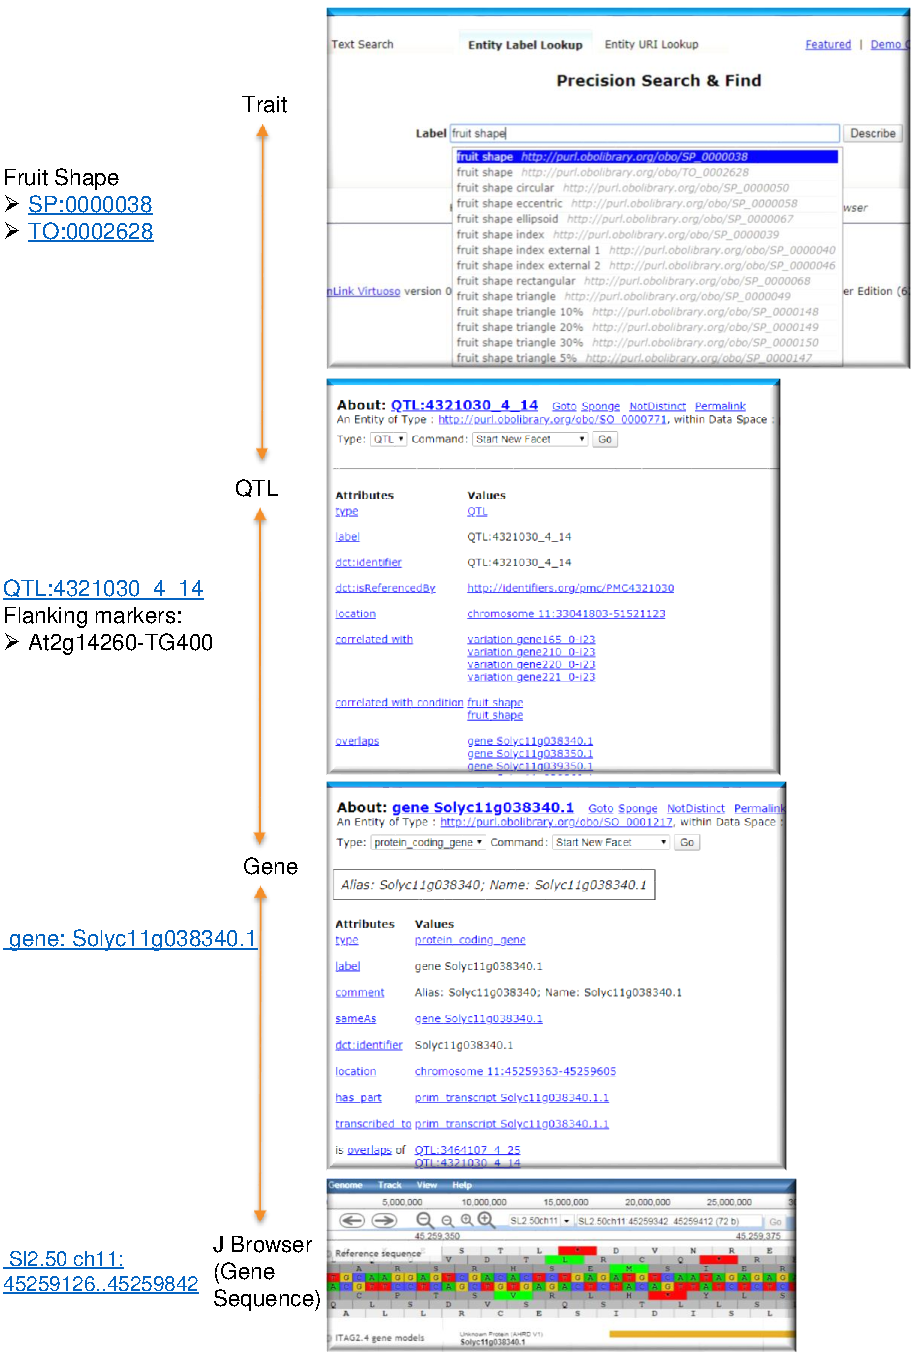
\includegraphics[width=\textwidth]{Figure2.pdf}
\caption{Browsing trait-gene associations on the faceted browser for the example trait “fruit shape”.}
\label{Figure2}
\end{figure}

\newpage


\subsection{Exemplary Data Queries via SPARQL and API}

\begin{enumerate}[label=(\Roman*),leftmargin=*,labelsep=0mm]

\item \textbf{\hl{SPARQL query to list QTLs,} %MDPI: is the bold necessary? same as below. yes, this highlights a possible user interaction
 associated gene IDs and GO annotations related to an example trait ``fruit shape'' (SP:0000038).}


Similar to the manually browsed query in Figure~\ref{Figure2} with a user interface, Figure~\ref{Figure3} exemplifies a way to write the query of trait-gene associations. This query yields QTLs and candidate genes including GO terms (molecular function and biological process only) for the trait “fruit shape” (SP:0000038).
\vspace{-2mm}
\begin{figure}[H]
\centering
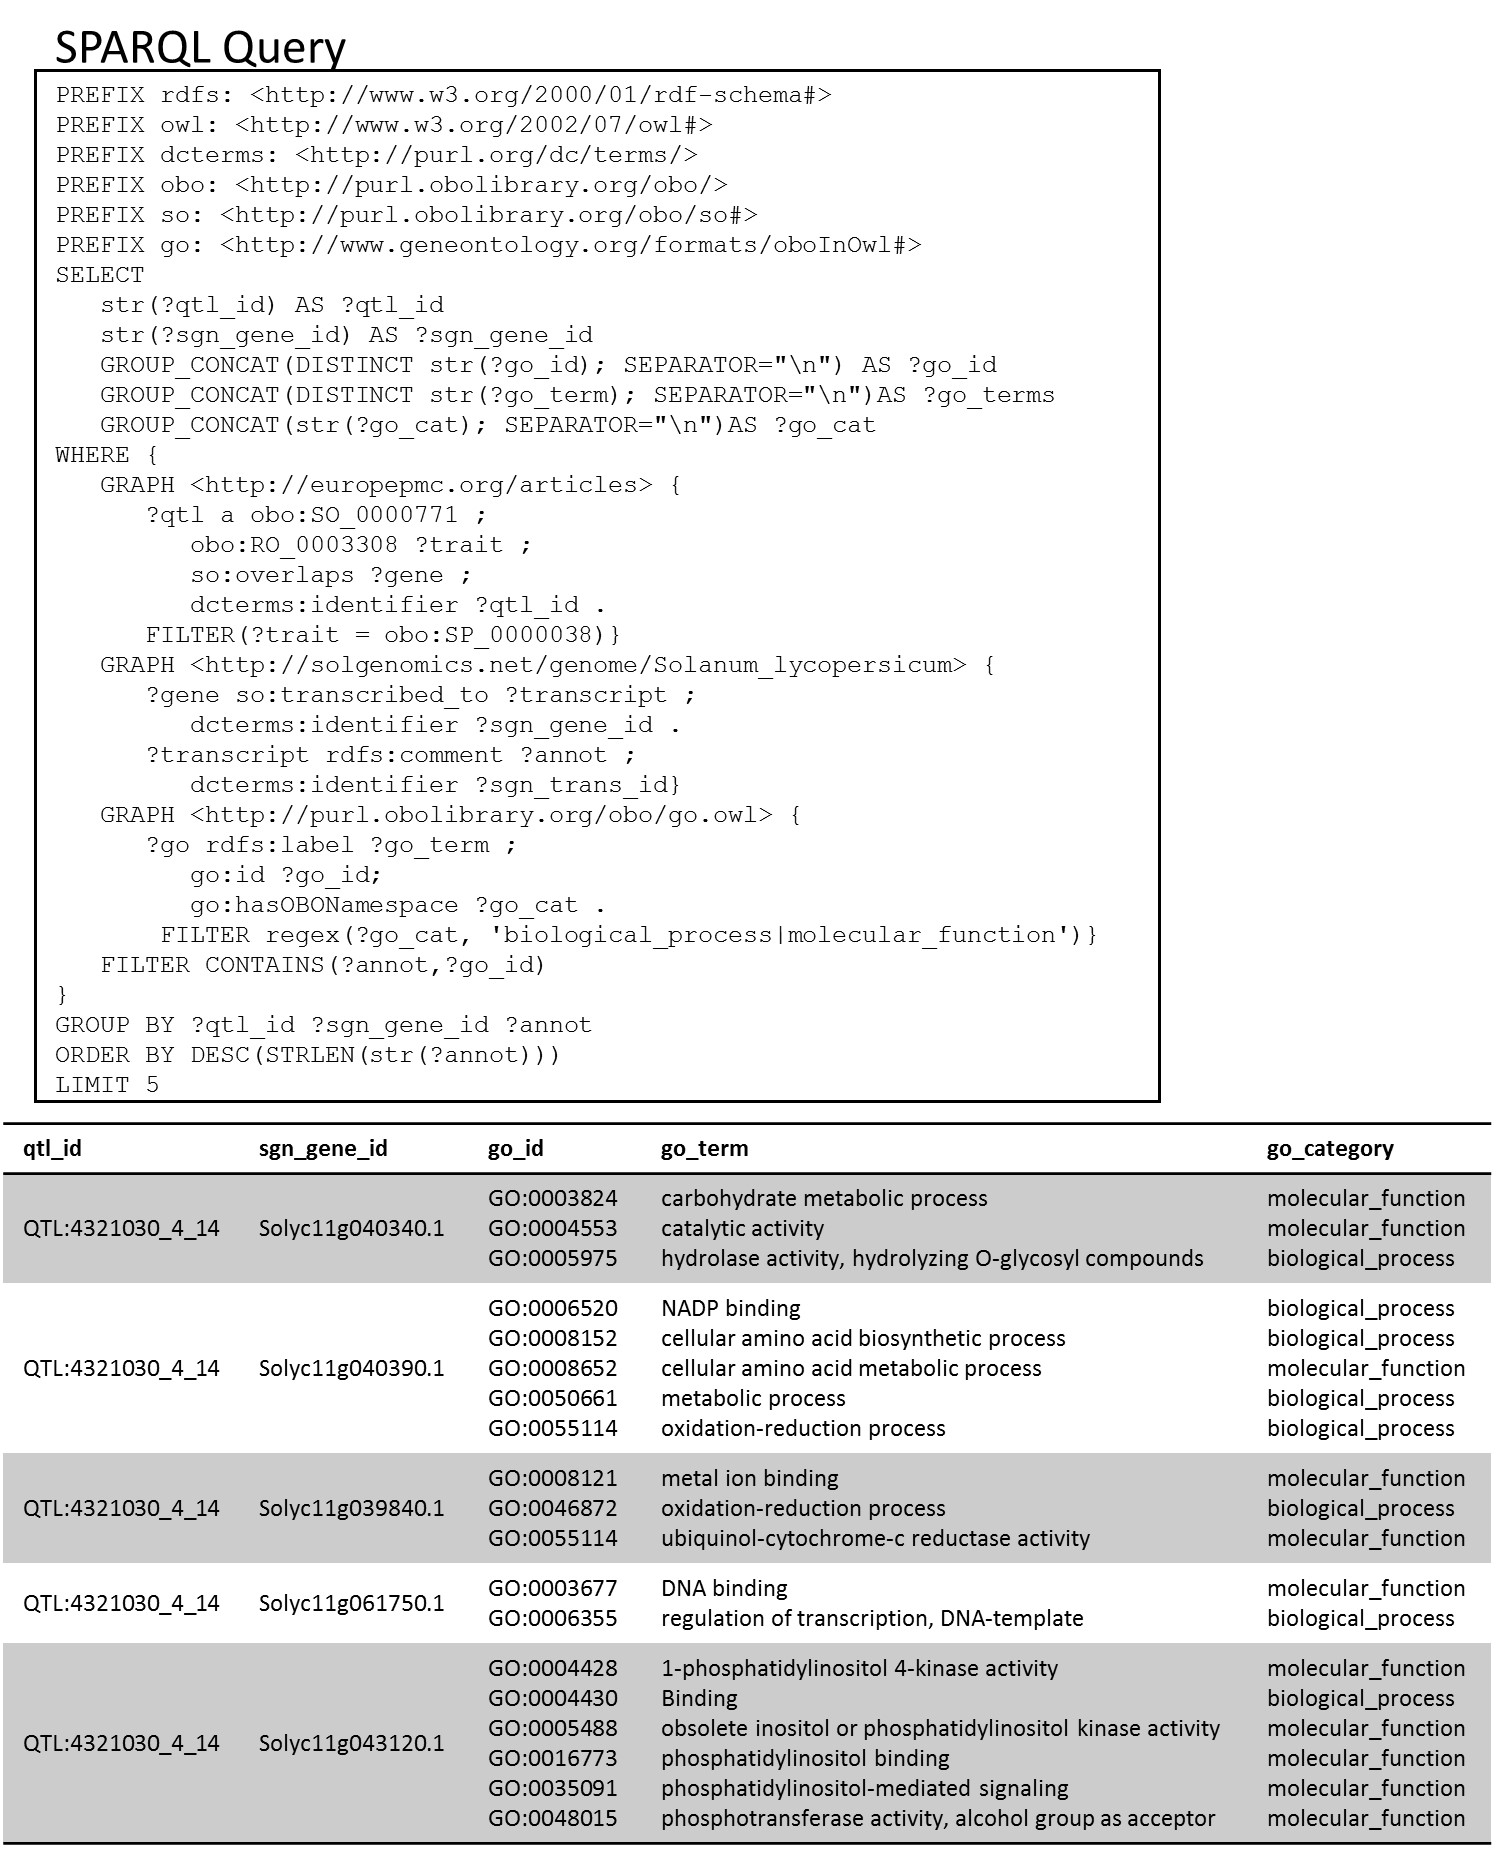
\includegraphics[width=0.78\textwidth]{Figure3.jpg}
\caption{Input and output of the SPARQL query to list QTL, associated gene IDs, and~Gene Ontology (GO) annotations related to a trait (example fruit shape (SP:0000038).  }
\label{Figure3}
\end{figure}
\item \textbf{\hl{SPARQL query to list} %MDPI: is the bold necessary? same as below. Yes, this highlights a possible user intereaction
 genes/proteins annotated with GO terms related to both “fruit” and~“ripening”.}




SPARQL query in Figure~\ref{Figure4} highlights a way to do textual search over the annotations of genes/proteins. With~the help of bag-of-words based regular expressions, we query genes and proteins containing GO annotation with the words “fruit” and “ripening”. The~resulting output is the list of genes/proteins involved in the biological process called fruit ripening (i.e.,~represented in the GO ontology with the id GO:0009835).\vspace{-2mm}
\begin{figure}[H]
\centering
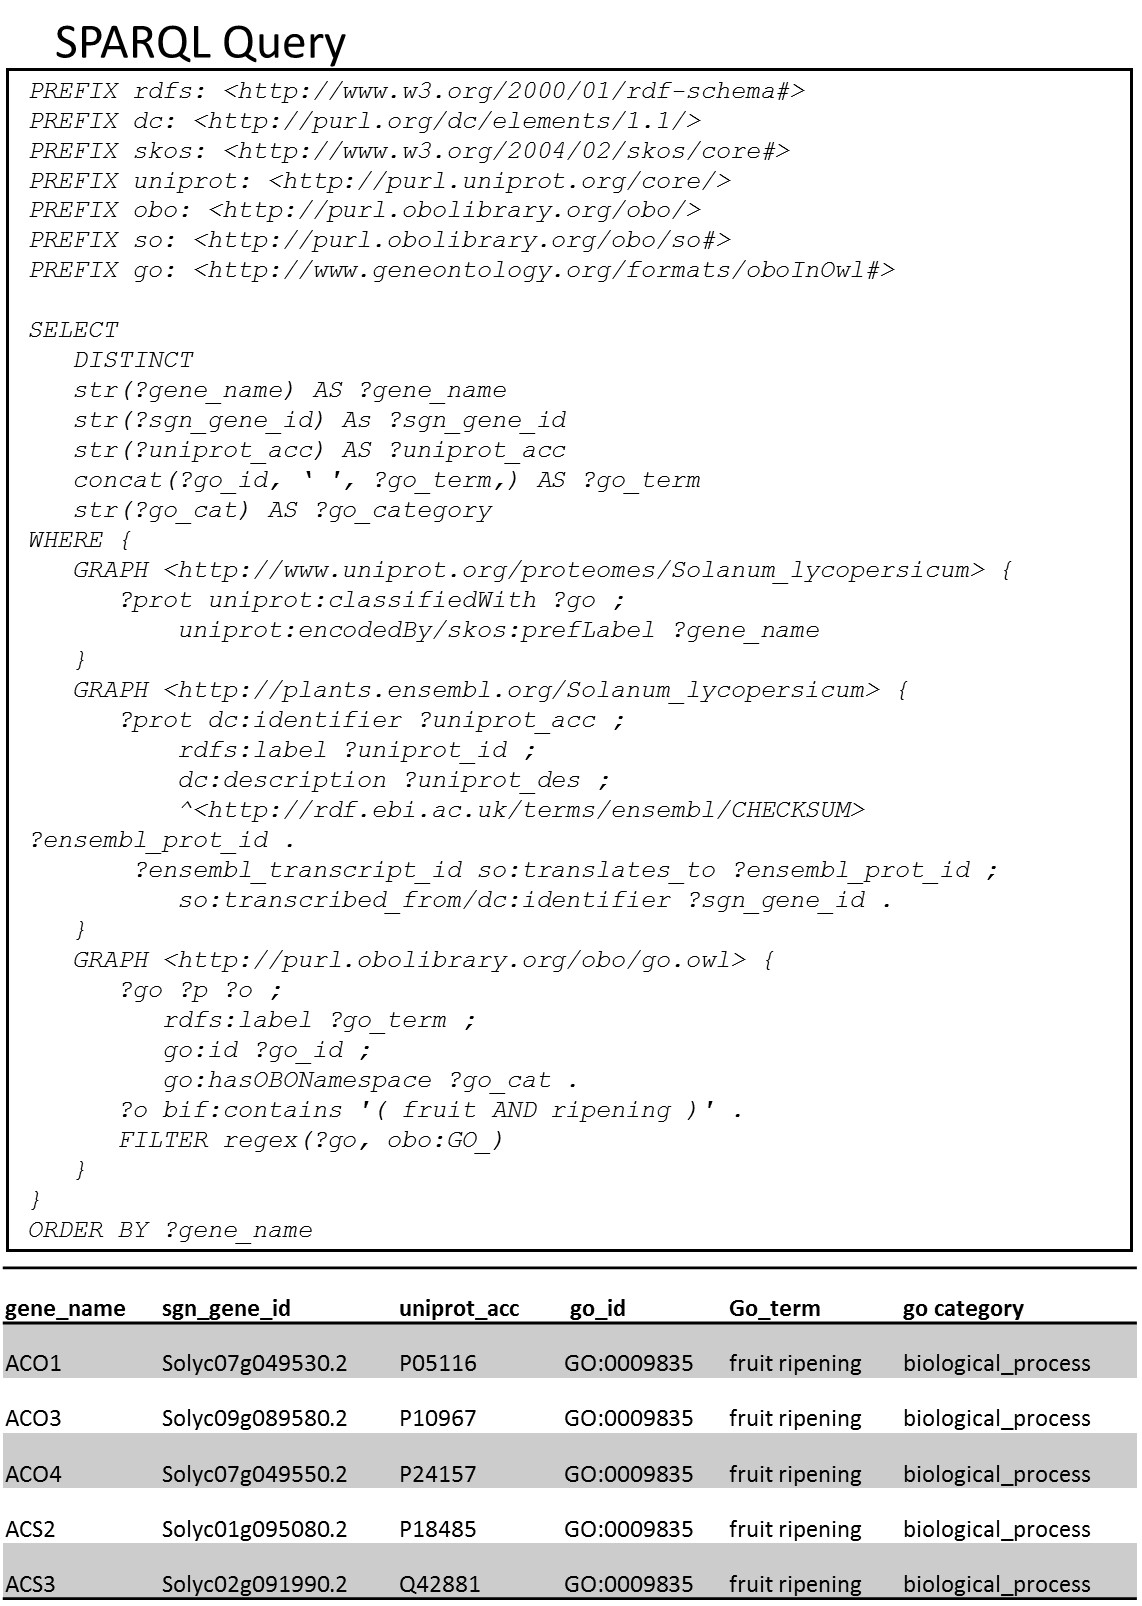
\includegraphics[width=0.57\textwidth]{Figure4.jpg}
\caption{Input and output of the SPARQL query to list genes/proteins annotated with GO terms related to both “fruit” and “ripening”. Searching for text matches (regular expressions) in the SPARQL query has been done with the help of virtuoso's bif:contains~predicate.}
\label{Figure4}
\end{figure}

\item \textbf{Comparison of (wild) tomato genome graphs using the RESTful API.}





Pbg-ld can be used to check genomic features across various biological databases. This can be done either by writing a SPARQL query against the endpoint or via API call /countFeatures of pbg-ld, with~the genomic graph as a parameter. For~example, Pbg-ld can counts the genomic features annotated in the \textit{S. lycopersicum} genome according to Ensembl Plants \url{https://plants.ensembl.org/Solanum_lycopersicum} or according to SGN (\url{http://solgenomics.net/genome/Solanum_lycopersicum}) and annotations in the \textit{S. pennelli} genome according to SGN (\url{http://solgenomics.net/genome/Solanum_pennellii}). We compare the differences between the genomic features of the tomato graphs in a bar chart (Figure \ref{Figure5}). It’s evident that there are a total of \hl{33785}  %Please check if commas should be added within the five-digit numbers? This is Dutch style formatting, but we can adhere to the journal standards by adding a comma to the five-digit numbers.
protein coding genes in Ensemble Plants, whereas there are \hl{34725} protein coding genes in the SGN graph. There are about 940 unique genes in the SGN database that are not mentioned in the Ensembl Plants database. Furthermore, the~results also highlight that genetic markers are included in SGN but not in Ensembl Plants while the latter database contains RNAs.    
On the one hand, where pbg-ld can be used to compare databases, pbg-ld can also be used to compare genomic data of different species of the same family. \textit{S. pennellii} is a wild tomato species that is relatively distant from the domesticated  \textit{S. lycopersicum}. Because~of \textit{S. pennelli}’s extreme stress tolerance, unusual~morphology, and~a genome sequence 119 Mb more than \textit{S. lycopersicum}, it~is an important donor of germplasm for the cultivated tomato. While comparing the genomic features \textit{S. lycopersicum} in SGN vs. \textit{S. pennelli} in SGN in Figure~\ref{Figure5}, the~number of genomic features in \textit{S.~pennellii} is on average 1.5 times greater than that of \textit{S. lycopersicum}.  
\end{enumerate}
% start a new page
\newpage
% change it to landscape
\paperwidth=\pdfpageheight
\paperheight=\pdfpagewidth
\pdfpageheight=\paperheight
\pdfpagewidth=\paperwidth
\newgeometry{layoutwidth=297mm,layoutheight=210 mm, left=2.7cm,right=2.7cm,top=1.8cm,bottom=1.5cm, includehead,includefoot}
\fancyheadoffset[LO,RE]{0cm}
\fancyheadoffset[RO,LE]{0cm}
 %%%%%%%%%%%%%%%%%%%%%%%%%%%%%%%%%%%%%%%%%%%%%%%

%\begin{landscape}
%\begin{sidewaysfigure}[htp!]
\begin{figure}[H]
\centering
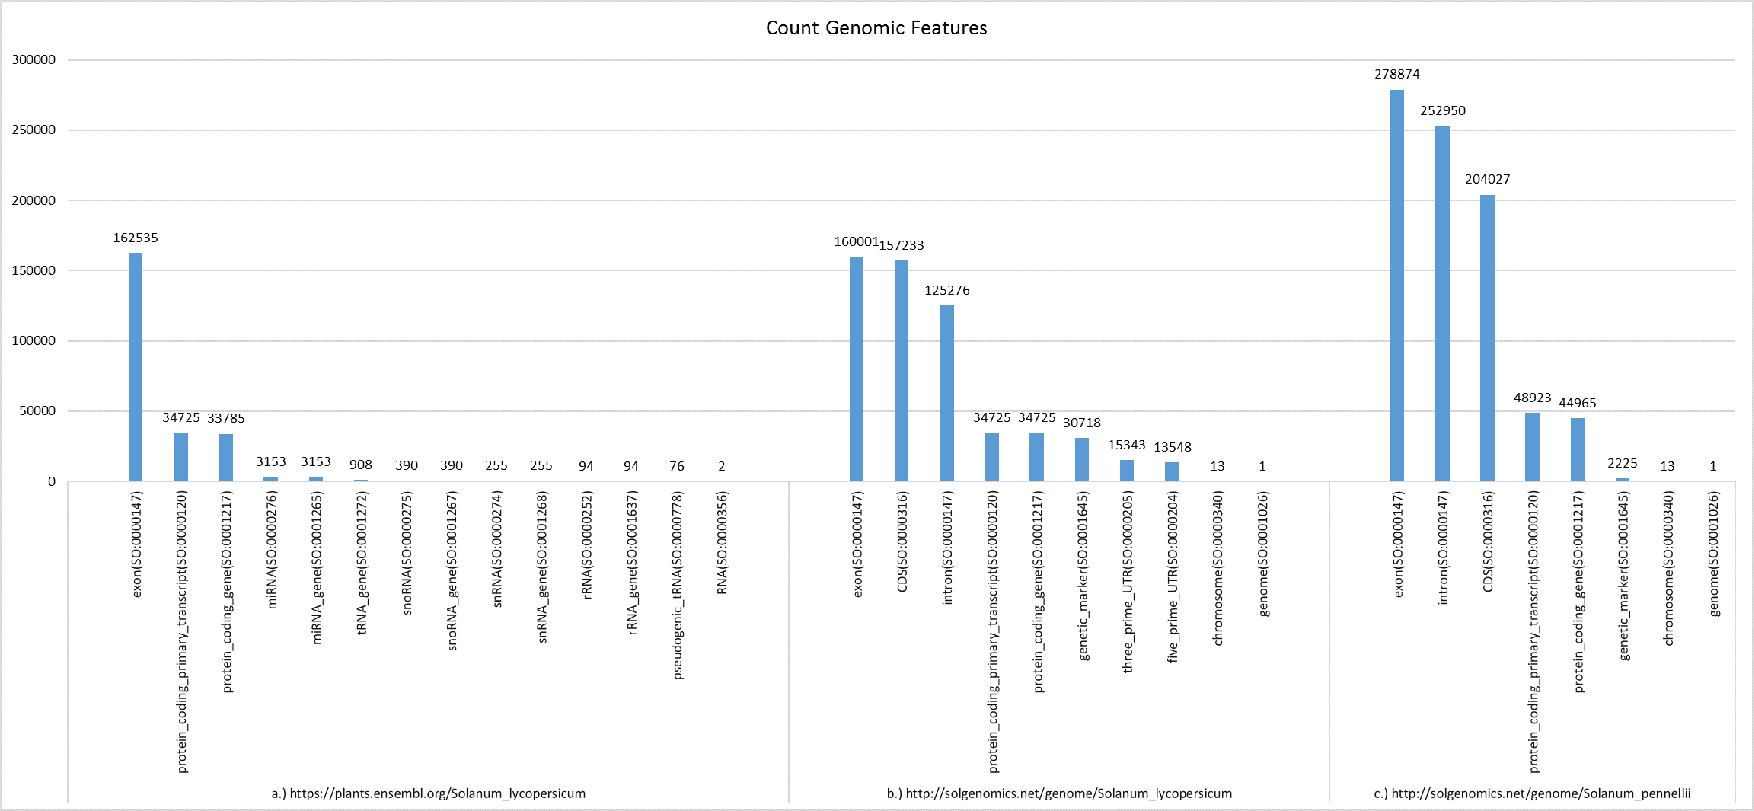
\includegraphics[scale=0.8]{Figure5.pdf}
\caption{Bar charts of genomic feature counts for three Solanum genomes (graph IRIs):
Ensembl: \emph{\hl{S. lycopersicum} %MDPI: we revised it to italic, same as below highlight, please confirm. Correct.
} (\url{http://plants.ensembl.org/Solanum_lycopersicum});
SGN:  \emph{\hl{S. lycopersicum}} (\url{http://solgenomics.net/genome/Solanum_lycopersicum});
SGN: \emph{\hl{S. pennellii}} (\url{http://solgenomics.net/genome/Solanum_pennellii}). {The data were obtained through the pbg-ld Web API} \href{http:\/\/localhost:8088\/api-local\/\#\/Count\%20genomic\%20features\/get_countFeatures}{/countFeatures} {endpoint.}}
\label{Figure5}
\end{figure}
%\end{sidewaysfigure}
%\end{landscape}

%%%%%%%%%%%%%%%%%%%%%%%%%%%%%%%%%%%%%%%%%%%%%%%
% change everything back
\newpage
\restoregeometry
\paperwidth=\pdfpageheight
\paperheight=\pdfpagewidth
\pdfpageheight=\paperheight
\pdfpagewidth=\paperwidth
\headwidth=\textwidth




\subsection{Biological Use Case 1: Comparative Genomics to Study Tomato Fruit Shape and Potato Tuber Shape}

For this use case, we used the pbg-ld endpoint (APIs) with a Jupyter Notebook~\cite{kluyver2016jupyter} to study the difference in the genetic mechanism underlying fruit shape in tomatoes and tuber shape in potatoes~\cite {Noteboook:example1}.

Both tomato fruits and potato tubers can have a genetically determined wide variation in their shape, for~example elongated and round. The~candidate gene \textit{Solyc10g076180} (SlOFP20 is a member of the OVATE Family Protein (OFP)) on chromosome 10 of the reference tomato genome (Heinz 1706) and is one of the determinants of round fruit shape. However, this gene does not have an ortholog in the reference potato genome (DM), which has very elongated tubers~\cite{wu2018common}. In~this use case, first, we~query and compare the QTL regions on chromosome 10 in tomato and in potato. This QTL regions are associated with round shape in tomato fruits and predominantly elongated shape in potatoes. We classify these genes in three categories \hl{(a)} %MDPI: should it be (a). Yes, this is correct, for clearity we changed tables into categories before this.
 genes that are unique in tomato (b) genes that are unique in potato (c) genes that are common to both species (see Table~\ref{chap4:T1}). Furthermore, we check the GO annotations as well as orthologs in all these genes. Three genes (\textit{Solyc10g076170.1}, \textit{Solyc10g076190.1}, \textit{Solyc10g076180.1}) are present in class (a) which indicates that they are unique in tomato. Out of these genes; the \textit{Solyc10g076170.1} gene was removed from the latest UniProt release. \textit{Solyc10g076190.1} is a peroxidase gene (that is also common in class (b) and class (c)) in our Table~\ref{chap4:T1} and \textit{Solyc10g076180.1} is the only unique member of the OVATE family. Genes in class (b) are all peroxidase genes and the class (c) contains several genes coding for peroxidases and one gene involved in lipid~transport. 



 According to our analysis the candidate gene \textit{Solyc10g076180.1} does not have a  corresponding ortholog in the potato DM reference genome in the same QTL region on chromosome 10. Therefore, with~the help of our tool we tried to explore this further, and~retrieve a knowledge network based on homologs of our candidate gene. This homologs network is retrieved with a nested query, in~which we first locate all paralogs of \textit{Solyc10g076180.1} gene in the tomato genome and then find orthologs of these genes in the potato genome (Figure \ref{Figure6}). With~the help of this nested query analysis, we were able to find 10 OFP (green) genes in potato and 11 genes (red) in tomato. One less potato gene (green) node is due to the missing OFP20 gene in the studied~QTL. 
 
 
 \unskip
\begin{figure}[H]
\centering
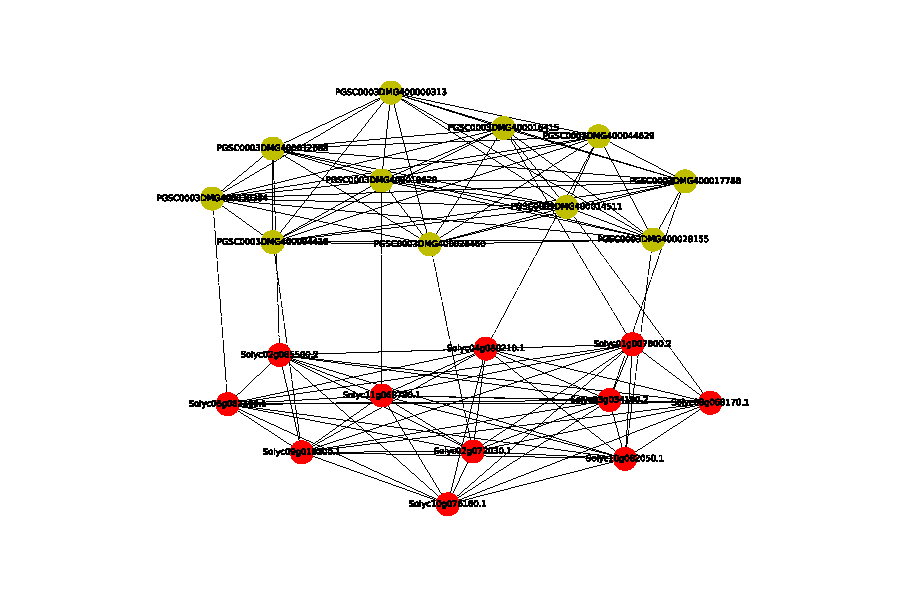
\includegraphics[scale=1.25]{Figure6.pdf}
%\captionsetup{type=figure,width=0.85\textwidth}
\caption{A network of \textit{Solyc10g076180.1} homologs in tomato (red) and potato (green) including paralogous (solid) and orthologous relations (dotted). There is no ortholog of OFP20 gene in~potato.}
\label{Figure6}
\end{figure}
\unskip

\begin{table}[H]
\centering
\caption{\textbf{\hl{Table comparing genes} %MDPI: is the bold necessary? and please provide an editable table. No, the bold is not necessary, the first author is not available and will not be able to prepare editable tables right now
 in QTLs associated with (tomato) fruit shape and (potato) tuber shape.} Three classes represent (a) Genes unique in tomato;  (b) Genes unique in potato (c) Genes mapped in both species. Each row contains a geneID, GO annotations, orthologs inside QTL region, and~orthologs outside the QTL regions. The~query shows that only three genes are unique in tomato (i.e., \textit{Solyc10g076190.1}, \textit{Solyc10g076170.1}, \textit{Solyc10g076180.1}).
}
%\captionsetup{width=\linewidth,skip=8pt}
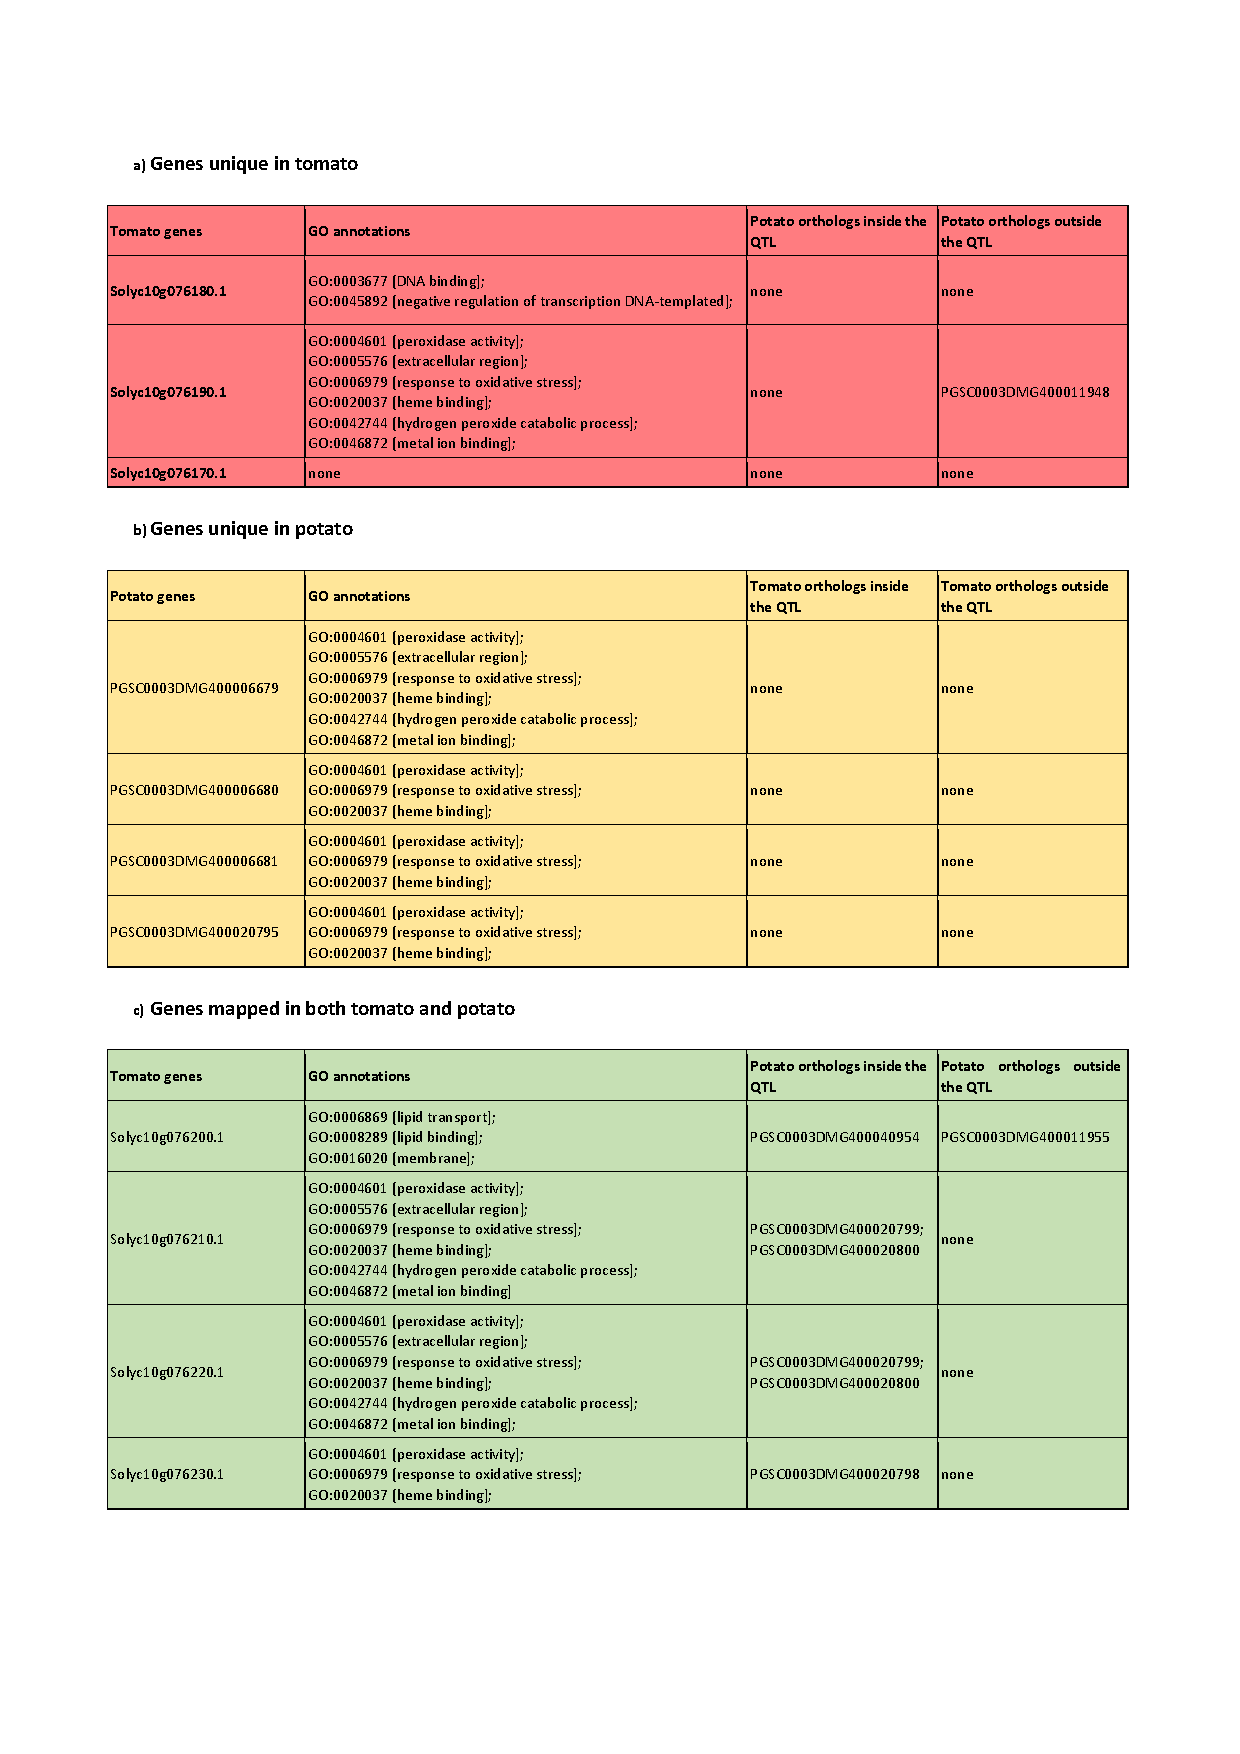
\includegraphics[scale=.88]{Table1.pdf}
\label{chap4:T1}
\end{table}

Out of the remaining 10 OFP genes in potato, PGSC0003DMG400028155 is located on chromosome 10 in the region 56030393-56031156. However, this region is 6.7Mb away from the studied QTL region and thus seems unlikely to harbor the  determinant candidate~gene. 

\subsection{Biological Use Case 2: Prediction of Candidate Genes in Tomato QTL Regions with Functional Annotations and Evolutionary Analysis, by~Using pbg-ld and QTLSearch}

Predicting candidate genes for QTL regions is a key objective in plant genetics and breeding. However, a~single QTL region can contain many genes. Mining candidate genes from such a QTL region could be done using existing knowledge of structural and functional gene annotations. In~this use case we aim to develop, illustrate, and~analyze a seamlessly integrative workflow that uses linked genomic-data and prioritization pipelines to predict candidate genes within QTL regions for metabolic traits of tomato. Metabolic composition of a tomato is directly associated with its nutritional value, taste, aromas, and~quality~\cite{ballester2016identification}. Metabolomic research studies in the past, have been able to predict functional characteristics of metabolites in the life-cycle of a plant. For~example, volatiles are known to play an important role in the defense mechanism of plants against pathogens, where they serve as airborne signaling molecules to induce a defense response in other plant parts or neighboring plants~\cite{shulaev1997airborne}. Similarly, other metabolites like soluble solids (glucose, fructose, and~sucrose) contribute to the sweetness of a fruit~\cite{luengwilai2010comparison}. Lycopene is a carotenoid compound found in tomatoes which contributes to the nutritional value of a tomato and the red pigment in tomatoes responsible for fruit-color~\cite{di1989lycopene}. Similarly, terpenoids play a role in attracting pollinators~\cite{falara2011tomato}.

Finding candidate genes within QTL regions for the trait of interest, using computational approaches is a major challenge in plant bioinformatics. Several tools have been developed in the past that tried to prioritize candidate genes based on existing knowledge. QTLSearch is a software tool that searches for candidate causal genes in QTL studies by combining Gene Ontology annotations across many species and leveraging hierarchical orthologous groups~\cite{warwick2018prioritising}. QTG-Finder is a recently published article that uses a machine learning model to prioritize candidate genes in using function annotation, co-function network, and~paralog copy number~\cite{lin2019qtg}. However, both these tools have been developed in \textit{Arabidopsis thaliana} and rice (\textit{Oryza sativa}) and it is difficult to use and test these tools in other species like tomato and potato. QTLSearch uses the HOGProp algorithm that requires access to hierarchical orthologous groups available in OMA browser~\cite{schneider2007oma}, to~score candidate genes based on trait-related GO terms. As~the OMA browser data graph is cross-referenced in Uniprot, which is part of pbg-ld, the~QTLSearch algorithm can be tested for tomato/potato data with the help of~pbg-ld.



Figure~\ref{Figure7} illustrates a prediction to candidate genes workflow within a QTL region for the trait of interest, using function annotations and evolutionary genomics data. Input to this workflow is either a QTL region (containing physical location or a genetic location) or a trait of interest. If~the input parameter is a trait of interest, the~Pbg-ld database retrieves all QTL locations for that trait in tomato. After~receiving the QTL inputs, this workflow queries the set of all genes occurring within this QTL region. For~every gene, this workflow retrieves a set of all GO terms as well as all orthologs and paralogs of these genes. These genome annotations are served as input to the QTLSearch pipeline which uses the Hogprop algorithm. HogProp algorithm assigns scores to every Gene within a QTL region. It uses GO terms which relate to the trait of interest and GO terms which relate to the genes within a QTL region to assess the distance of these functional annotations along gene phylogenies. This~workflow has been developed in a Jupyter Notebooks, provided in Reference \cite{Noteboook:example2}. It is a modular framework in which data is fetched from multiple data sources and can also accommodate new analysis modules as they are being developed by our group or the scientific~community.
\begin{figure}[H]
\centering
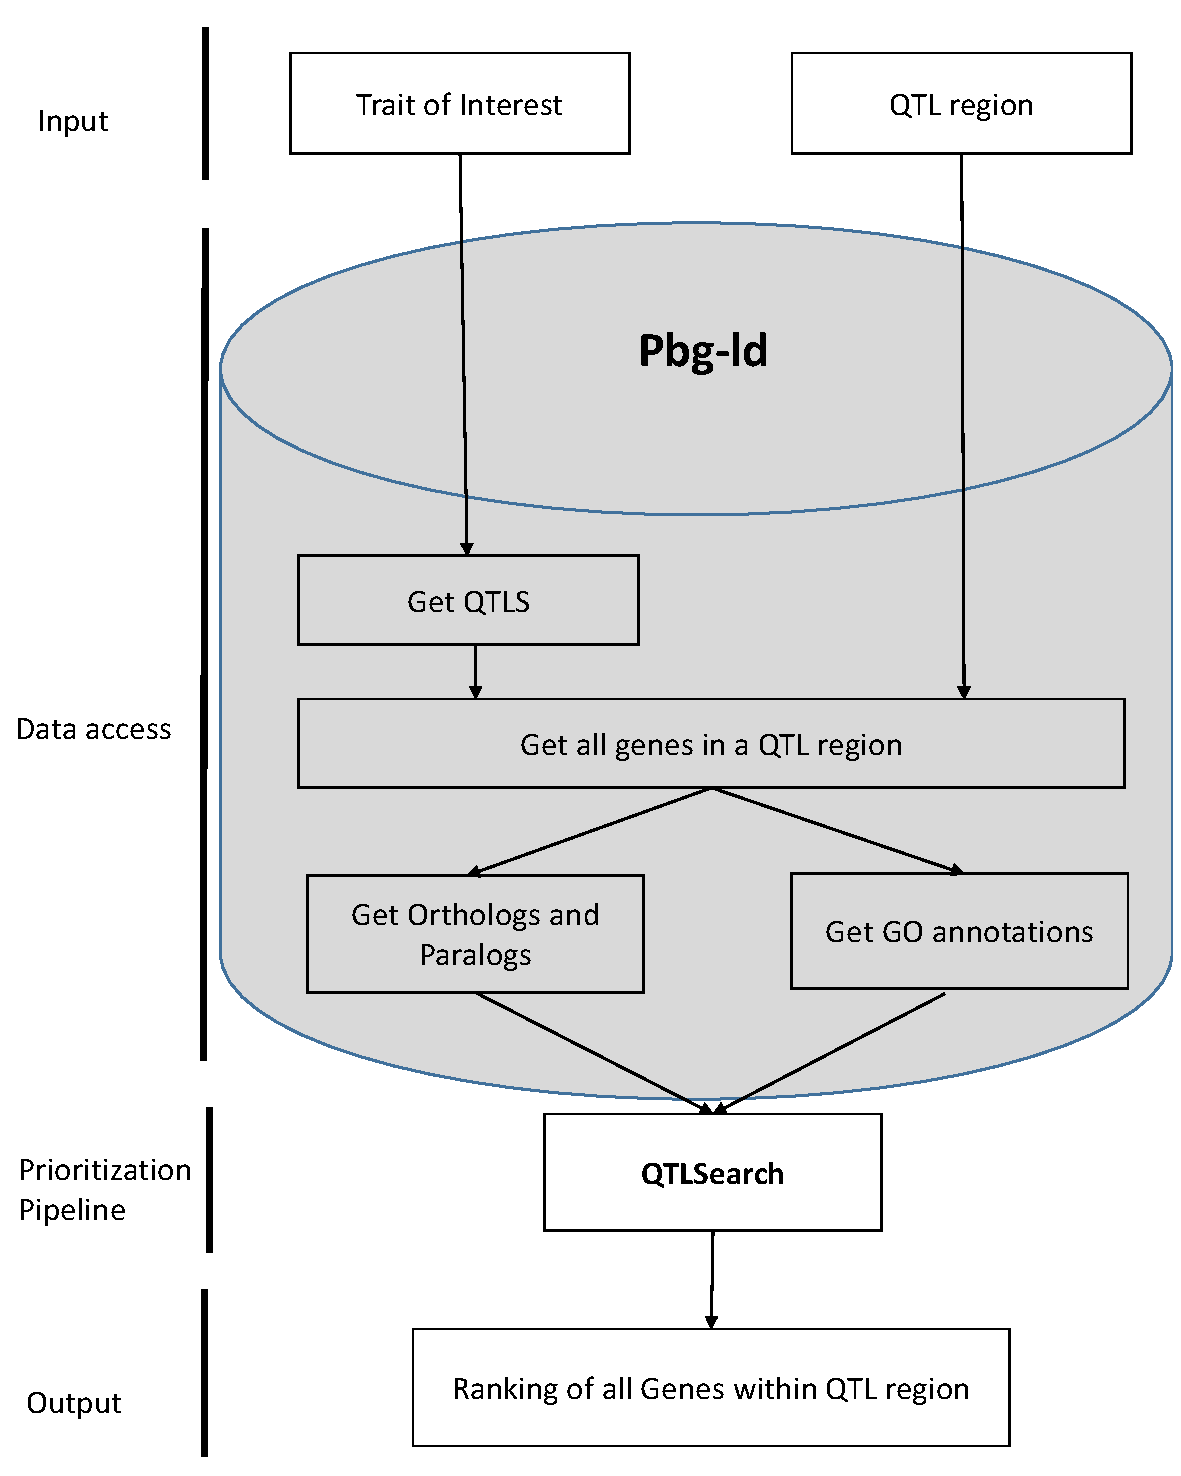
\includegraphics[scale=0.60]{Figure7.pdf}
\caption{A workflow to predict candidate genes in a QTL region for the traits of~interest.} \label{Figure7}
\end{figure}

To test the usability of our workflow in predicting candidate genes for metabolic traits, we~selected 5 QTLs for different metabolic traits that is, Brix/soluble solids, lycopene beta-cyclase activity, 2-phenylethanol/phenylacetaldehyde, (See Table~\ref{c5:tab1}). Out of the selected 5 QTLs for metabolic traits, 3~QTLs which relate to the following traits, soluble solids, lycopene beta-cyclase activity and phenolic compounds (2-phenylethanol, phenylacetaldehyde), have known candidates. Further, these~candidate genes are already annotated with related GO terms in publically available databases like UniProt. While, for~one of the QTL regions which relates to terpenoids, Terpene synthase is a known candidate gene, however, Terpene synthase is not annotated with GO terms which show an association with the trait of interest (i.e., terpenoids). The~2 GO terms related to this gene are DNA binding and DNA methylation. Lastly, for~the QTL region selected for volatile compounds (i.e.,~3-methylbuthanal, 3-methylbuthanol) there are no well-known candidate genes in the QTLs that had experimentally proven~significance. 

\begin{table}[H]
\centering
%{2cm}
%\captionsetup{width=\linewidth,skip=8pt}
\caption{\textbf{\hl{A selected set of} %MDPI: is the bold necessary? No, the bold can be removed.
 5 QTLs for metabolic traits in tomatoes.} These 5 QTLs are used as test-cases  to analyse the prediction power of the underlying~workflow.}
\label{c5:tab1}
{
%\begin{adjustwidth}{-0.5cm}{}
%\setlength{\tabcolsep}{2pt}
{
\scalebox{.86}[.86]{\begin{tabular}{c  c  c  c  c  c }
\toprule
\textbf{Traits of Interest} & \textbf{GO Annotations} & \textbf{Chromosome} & \textbf{Location} & \textbf{Candidate Genes} & \textbf{References} \\
%\midrule
\midrule
%&&&&&\\[0.5cm]
Total soluble solids (Brix) & \makecell{ GO:0006094, \\ GO:0046370, \\ GO:0046369, \\ GO:0005985, \\ GO:0015770 } &    9 &    3474710 &    Lin5 & \cite{fridman2002two} \\    %[2 cm]
\midrule
\makecell{Carotenoid compounds\\ (Lycopene beta-cyclase activity)} & \makecell{ GO:0045436, \\
GO:0016117} & 6 & \makecell{Solyc06g073470\\ Solyc06g083850.3} & Soly06g074240.1 & \cite{bouvier2000identification} \\ %[2 cm]
\midrule
\makecell{Polyphenolic compounds\\ (2-phenylethanol\\ \& phenylacetaldehyde)} &    \makecell{ GO:0016747, \\ GO:0102387, \\ GO:0018449, \\ GO:0004029, \\ GO:0008957, \\ GO:1990055, \\ GO:0050177, \\ GO:0018814} & 8 &    55068565-63267130 &    LePAR%CT77 / CT148 
& \cite{tadmor2002identification}\\    %[2 cm]
\midrule
Terpenoid compounds & \makecell{ GO:0003677, \\ GO:0045893} & 1 & 86142248-86467672 & Terpense synthase & \cite{falara2011tomato} \\    %[2 cm]    
%Volatile compounds ( eugenol, methyl salicylate, guaiacol ) & \makecell{GO:0042855, \\  GO:0042856, \\ GO:0042854, \\ GO:0080031 \\ GO:0052689} & 9 & 69082273-69353332 &    ? &    \cite{tieman2010functional}\\ [1 cm]
\midrule
\makecell{Volatile compounds\\ ( 3-methylbuthanal, \\3-methylbuthanol)} & \makecell{GO:0046568, \\ GO:0018455, \\ GO:0052676} & 3 & 69685329-71362039 & ? & ?\\ %[1 cm]
%\hline
\bottomrule
\end{tabular}}
}
%\end{adjustwidth}
}
\end{table}

The top 3 predicted candidate genes for each trait with the help of our pipeline are reported in the Table~\ref{c5:tab2}. 

One of the most extensively studied metabolic traits in tomato is the total soluble solids content in fruits (i.e., TSS or Brix) \cite{fridman2002two}. We selected 5 GO terms related to these metabolites and Brix trait (see Table~\ref{c5:tab2}) and fed it to the QTLSearch pipeline in our workflow. Previously known studies have identified multiple QTLs that are associated with the Brix trait in tomatoes~\cite{haggard2015multiple}. Out of the many known QTL locations, the~most significant QTL is located on chromosome 9, containing Lin5 as the popularly known candidate gene for Brix trait~\cite{fridman2002two}. Table~\ref{c5:tab2} highlights the top 3 genes predicted from our workflow for the Brix QTL region from 3374710 to 3574710 on Chromosome 9. Lin7 and Lin5 were the top predicted genes related to this trait. Both these genes are from a homologous family and are known to be associated with Brix. The~score of these 2 genes is significantly higher than all other genes. We conclude that our pipeline performed well to predict the candidate genes for this~QTL. 

Carotenoid compounds are the primary determinants of tomato fruit color~\cite{marti2016tomato}. Carotenoids exert a broad range of functions which associate to photosynthesis, the~formation of pigments, antioxidant activities, and~being precursors to signaling molecules, including volatiles~\cite{giuliano2014plant}. Lycopene is a major carotenoid in tomato~\cite{shi2004antioxidative}. Lycopene occurrence with other bioactive compounds, like vitamin C, vitamin E, other carotenoids (a-carotene, beta-carotene, gamma-carotene, lutein), and~flavonoids is primarily associated with the color of a tomatoes. Lycopene beta-cyclase is a key enzyme occurring at the branch point of the carotenoid biosynthesis pathway and responsible for converting lycopene to beta-carotene. Lycopene beta-cyclase activity is also related to the total carotenoid content accumulated in the tomato fruit. The~major QTL region which is related to Lycopene beta-cyclase activity is found to be located on Chromosome 6 between the region 45280179--49150528~\cite{cunningham1996functional}. Here we analyzed the prediction of candidate genes for Lycopene beta-cyclase activity with the help of our developed workflow. 2 GO terms that relate to lycopene beta-cyclase activity were selected for inclusion in our workflow. Previous known studies suggest that lycopene cyclase (LCY) is a known candidate gene related to this trait. In~some databases, lycopene cyclase (LCY) is also annotated as neoxanthin synthase (NSY) as these are genes that are closely related carotenogenic enzymes belonging to the same family. Table~\ref{c5:tab2} shows the results from the workflow, containing the top 3 genes predicted for this QTL region on Chromosome 6. NSY was ranked at the top of the list and has a score significantly higher than all other genes. Here also, we can conclude that our workflow performed as~expected. 

Phenolic derivative compounds like  2-phenylethanol, phenylacetaldehyde have a great impact on the aroma of a tomato~\cite{tadmor2002identification}.~Several QTL locations related to phenolic compounds have been identified in the past out of which, a~major QTL region on chromosome 8 mapped by the markers, TG330-CT77 and TG330-CT148 is associated with the accumulation of 2-phenylethanol and phenylacetaldehyde (having genomic coordinates 55068565-63267130) \cite{rousseaux2005qtl}. Additionally, two putative proteins, 2-phenylacetaldehyde reductases proteins (LePAR1 and LePAR2) are known candidates, which catalyze the conversion of 2-phenylacetaldehyde to 2-phenylethanol~\cite{tieman2007tomato}. Both these proteins are members of a reductase/dehydrogenase family. Table~\ref{c5:tab2} illustrates the top 3 genes predicted from our pipeline for these phenolic compounds on Chromosome 8. \textit{Solyc08g068190.2} was the top predicted gene related to this trait. Although~we are not sure if this gene is the same as LePAR1 and LePAR2, this~gene belongs to the same aldehyde dehydrogenase family. Therefore our workflow could detect the causal gene within this QTL~region. 

A major QTL related to Terpenoids has been mapped on chromosome 1 with the genomic coordinates of 86142248--86467672~\cite{zhang2015genome}. Proteins of the Terpene synthase (TPS) family and TPS gene are the expected candidate genes associated with Terpenoids. 5 of the TPS-a subclade genes (TPS31, TPS32, TPS33, and~TPS35) occur in close proximity within this QTL. Table~\ref{c5:tab2} highlights the top 3 genes predicted from our pipeline for this QTL. Our results suggest that the gene \textit{Solyc01g095030.2}, which is a MYB transcription factor, is the causal gene for this QTL region. This is possibly the wrong prediction. The~reason for our pipeline to give a wrong prediction here could be that there is no term present in the GO ontology that directly related to Terpenoids. Further, because~of this missing GO annotation terms, Terpene synthase is not been well annotated with its function, which makes it difficult for our workflow to detect it as a high ranking gene for the Terpenoids~trait. 

Volatile compounds like 3-methylbuthanal, 3-methylbuthanol influence the flavor, sensory changes, and~defense mechanism of tomato fruits~\cite{socaci2014chemometric}.~A~major QTL related to the volatile compounds (3-methylbuthanal, 3-methylbuthanol) has been mapped on chromosome 3 with the genomic coordinates of 69685329--71362039~\cite{rambla2016identification}. However, it is not known which candidate gene in this QTL is responsible for changes in the concentration of these volatile compounds. Our results suggest that the lactate dehydrogenase (LDH) gene is possibly a candidate gene for this~trait. 


{Out of the total 5 QTLs, our workflow performed significantly well in detecting candidate genes for the QTLs of soluble solids, lycopene beta-cyclase activity, and~phenolic compounds. Our workflow did not perform well in the detection of candidate genes within the QTL for terpenoids on chromosome 1. This is most probably due to the fact that this QTL region is not well annotated, and~there are no GO terms related to Terpenoids. Lastly, our workflow predicts a candidate gene called LDH, for~the previously unknown QTL region associated with volatile compounds.} 


QTLSearch, a~prediction pipeline for candidate genes in QTL regions is based on existing knowledge and evolutionary data (orthologs and paralogs). While the performance of QTLSearch is high with well-annotated data, it fails to perform well in detecting candidate genes for QTL regions where little is known. Hence, it’s still very challenging to infer about candidate genes with a less annotated QTL~region.


% start a new page
\newpage
% change it to landscape
\paperwidth=\pdfpageheight
\paperheight=\pdfpagewidth
\pdfpageheight=\paperheight
\pdfpagewidth=\paperwidth
\newgeometry{layoutwidth=297mm,layoutheight=210 mm, left=2.7cm,right=2.7cm,top=1.8cm,bottom=1.5cm, includehead,includefoot}
\fancyheadoffset[LO,RE]{0cm}
\fancyheadoffset[RO,LE]{0cm}
 %%%%%%%%%%%%%%%%%%%%%%%%%%%%%%%%%%%%%%%%%%%%%%%

%\begin{landscape}
\begin{table}[H]
\centering
%\captionsetup{width=\linewidth,skip=8pt}
\caption{Top 3 candidate genes found for the 5 selected metabolic traits (Brix/soluble solids, lycopene beta-cyclase activity, 2-phenylethanol/phenylacetaldehyde).}
\label{c5:tab2}
{\footnotesize
\setlength{\tabcolsep}{2pt}
%\resizebox{1.5\textwidth}{!}{
\begin{tabular}{ c  c  c  c  c  c  c }
\toprule
\textbf{Gene ID} & \textbf{Alias} & \textbf{UniProt ID} & \textbf{Protein Description} & \textbf{Chromosome Number} & \textbf{Location} & \textbf{Prioritization Score} \\
\midrule
%\midrule
%Solyc09g010090.2 &    LIN7 & Q8L4N2 & Cell-wall invertase & 3480545-3484159 & 0.193381 \\

\multicolumn{7}{c}{\textbf{Metabolic Trait 1: Brix/soluble solids}} \\
\midrule
Solyc09g010090.2 & LIN7 & Q8L4N2 & Cell-wall invertase & 9 & 3480545-3484159 & 0.202943 \\
%2
Solyc09g010080.2 & lin5 & Q9LD97 & Beta-fructofuranosidase insoluble isoenzyme 1 & 9 & 3475480-3479343 & 0.172502 \\
%3
Solyc09g010020.2 & - & K4CR31 & 1-aminocyclopropane-1-carboxylate oxidase & 9 & 3447416-3449839 & 0.043606 \\ %[5mm]
%4
\midrule
\multicolumn{7}{c}{\textbf{Metabolic Trait 2: Lycopene beta-cyclase}} \\
\midrule
Solyc06g074240.1 & NSY & K4C9E2 & Chromoplast-specific lycopene beta-cyclase & 6 & 45898227-45899723 & 7.399091 \\
Solyc06g073570.2 & 101245261 & K4C976 & Cytochrome P450 & 6 & 45361777-45364885 & 0.554559 \\
Solyc06g076160.2 & 101248306 & K4C9X6 & Cytochrome P450 & 6 & 47289151-47291972 & 0.471375 \\%[5mm]
\midrule
\multicolumn{7}{c}{\textbf{Metabolic Trait 3: 2-phenylethanol/phenylacetaldehyde}} \\
\midrule
Solyc08g068190.2 & 101257095 & K4CM43 & Aldehyde dehydrogenase & 8 & 57303048-57306002 & 3.702432 \\ 
Solyc08g076790.2 & 101246651 & K4CN39 & Cinnamoyl-CoA reductase-like protein & 8 & 60704895-60707948 & 0.009002 \\ 
Solyc08g068600.2 & 101264847 & K4CM83 & Decarboxylase family protein & 8 & 57730921-57733032 & 0.004473 \\%[5mm]
\midrule
\multicolumn{7}{c}{\textbf{Metabolic Trait 4: terpenoids}} \\
\midrule
Solyc01g095030.2 & 101257705 & K4AZP3 & MYB transcription factor & 1 & 86401425-86409205 & 20.423493 \\ 
Solyc01g094820.2 &  & K4AZM2 & ARID/BRIGHT DNA-binding domain-containing protein & 1 & 86227211-86231284 & 3.715449 \\ 
Solyc01g094800.2 & 101245796 & K4AZM0 & Chromodomain-helicase-DNA-binding protein 1 & 1 & 86208090-86220086 & 1.800694 \\%[5mm]
\midrule
\multicolumn{7}{c}{\textbf{Metabolic Trait 5: Volatile compounds}} \\
\midrule
Solyc03g122130.2 &  & K4BN11 & L-lactate dehydrogenase & 3 & 70079537-70082001 & 0.008994 \\ 
Solyc03g122140.2 & 101255867 & K4BN12 & L-lactate dehydrogenase & 3 & 70082466-70085406 & 0.008994 \\ 
Solyc03g122170.2 &  & K4BN15 & L-lactate dehydrogenase & 3 & 70091655-70095510 & 0.008994 \\ %[5mm]
\bottomrule
\end{tabular}
%}
}
\end{table}

%\vspace{2cm}

%\end{landscape}

%%%%%%%%%%%%%%%%%%%%%%%%%%%%%%%%%%%%%%%%%%%%%%%
% change everything back
\newpage
\restoregeometry
\paperwidth=\pdfpageheight
\paperheight=\pdfpagewidth
\pdfpageheight=\paperheight
\pdfpagewidth=\paperwidth
\headwidth=\textwidth

%%%%%%%%%%%%%%%%%%%%%%%%%%%%%%%%%%%%%%%%


\section{Discussion \& Conclusions}
The main objective of developing the pbg-ld platform was to improve the FAIRness of candidate gene identification in \textit{Solanaceae} %itelics added
species by providing (semantically) integrated genomics and QTL datasets available in public resources (i.e., UniProt, Ensembl Plants, SGN and Europe PMC) from a central~endpoint. 

Genomic knowledge discovery is often confronted by the challenges of data integration from a multitude of independent databases and research articles. For~discovering candidate genes with the help of large-scale data integration, there is a need to organize candidate data resources according to the FAIR data principles. The~core development in this research provides a linked data platform that semantically organizes and integrates genotypic and phenotypic data on \textit{Solanaceae} %itelics added
species according to these principles. Hence, this progress in digital science helps genomic datasets to be more findable, accessible, interoperable and~reusable.

After selecting various datasets and information relevant to candidate gene discovery, a~critical step in the knowledge discovery process is the transformation of data into a suitable data infrastructure. Biological data is complex and highly connected, for~example,~there is huge ambiguity in the names of genes, proteins, and~transcripts, hence semantic model with correct identifiers is required to differentiate them. Pbg-ld addresses the challenges of providing a semantic layer over most used datasets for candidate gene discovery in tomato and potato. A~critical step in our approach was the transformation of (semi-)structured or non-RDF data sources to inter-linked RDF graphs using existing and newly developed tools such as the QTM and SIGA.py. Further, FDP provides meta-data descriptions, which makes the user aware of the originating graph(s) to perform queries and to interpret the results. Different data access points provide flexibility for users who wish to analyze and/or visualize data on this platform. {Lastly, open accessibility of all the above mentioned tools used to generate and publish these data sets, offers the ability for the scientific community users to extend this tool for other crop species themselves.} 

Data sets are not static and constantly emerging over time. Pbg-ld combines open data from different third party resources such as Europe PMC, SGN, UniProt and Ensemble Plants. As~these data sets are not static a significant improvement in pbg-ld could be to automate the process of regular updates of the data sets. For~example, QTL information in pbg-ld is extracted from tables of scientific articles in Europe PMC via the QTM tool. However, QTL data graphs are static and require manual updates. Ideally, the~QTL data graph should be updated automatically, whenever a new QTL study is published. A~researcher is interested in retrieving the most newly published scientific articles in the domain of his/her research interests. Another improvement to the pbg-ld platform could be to enable (interactive) visualization of the knowledge~graphs.  

Complimentary to our developments, some similar plant-specific software and databases provide genotypic and phenotypic data sets in a semantically integrated way. KNETMiner is an open source software that integrates plant-specific biological data sets into a knowledge graph~\cite{hassani2017knowledge}. These biological data sets contain information related to genes, biological pathways, phenotypes and publications for many important crop species like wheat, rice, sorgum, potato, tomato, and so forth. Additionally, KNETMiner has an evidence-based gene ranking algorithm that ranks and visualizes this integrated data based on gene annotations. {However, in~ the current version of KNETMiner} \cite{Knetresources}{, it provides free-access to integrated data sets for only some important crops like wheat (\textit{Triticum aestivum}), rice (\textit{Oryza sativa}), \textit{Arabidopsis Thaliana}. The~integrated data set for other crop species like, tomato (\textit{S. lycopersicum}), potato (\textit{S. tuberosum}), and~sorgum (\textit{Sorgum bicolor}) is are not openly accessible. } Similarly, Planteome database~\cite{Cooper2018} provides gene annotations and phenotypes with the help of reference ontologies such as PO, TO, GO and ChEBI. Planteome is a user-friendly tool to query traits of interest, germplasm, and~putative candidate genes. However, it lacks QTLs, genetic markers and links to publicly available databases such as Ensembl Plants. Therefore, our linked data platform is a unique resource for \textit{Solanaceae} %italics added
species that provides access to available knowledge about genome annotations in public databases and scientific~literature.

Pbg-ld currently contains the gene models and the genetic markers based GFF files of the reference tomato genome (\textit{S. lycopersicum}), wild tomato  (\textit{S. pennellii}), and~the reference potato genome (\textit{S.~tuberosum}). However, other than these genomes, the~SGN database, for~instance also includes GFF files from other \textit{Solanaceae} %italics added
and closely related genomes species, such as reference genome of pepper (\textit{Capsicum annuum}) \cite{hulse2018reference}, eggplant (\textit{Solanum melongena L.}) \cite{hirakawa2014draft} and so forth. Converting these GFF files to RDF graphs and adding then to the pbg-ld would improve analyses based on comparative genomics. Nevertheless, a~big challenge in doing this type of analysis based on knowledge graphs is to have the mappings of biological entities (genes, proteins, etc.) among multiple species. There is a chance of having different identifiers in two related species, for~example, the~genomes of the reference sequence potato \textit{S. tuberosum} and wild type species \textit{M6} have both been sequenced, however, both use different sets of identifiers and the mapping of genes between these genotypes is not available. However, having~the data about cross references in these genes for both the genomes can give us better insights into underpinning certain gene functions with comparative~studies. 

To conclude, pbg-ld is an integrated resource for \textit{Solanaceae} species that provides access to available knowledge about genome annotations in public databases and scientific literature. This resource aids in the identification of candidate genes for complex traits using available knowledge in the databases and~literature.




%%%%%%%%%%%%%%%%%%%%%%%%%%%%%%%%%%%%%%%%%%

%\section{Results}

%This section may be divided by subheadings. It should provide a concise and precise description of the experimental results, their interpretation as well as the experimental conclusions that can be drawn.
%\begin{quote}
%This section may be divided by subheadings. It should provide a concise and precise description of the experimental results, their interpretation as well as the experimental conclusions that can be drawn.
%\end{quote}

%%%%%%%%%%%%%%%%%%%%%%%%%%%%%%%%%%%%%%%%%%
%\subsection{Subsection}
%\unskip
%\subsubsection{Subsubsection}

%Bulleted lists look like this:
%\begin{itemize}[leftmargin=*,labelsep=5.8mm]
%\item	First bullet
%\item	Second bullet
%\item	Third bullet
%\end{itemize}

%Numbered lists can be added as follows:
%\begin{enumerate}[leftmargin=*,labelsep=4.9mm]
%\item	First item 
%\item	Second item
%\item	Third item
%\end{enumerate}

%The text continues here.

%\subsection{Figures, Tables and Schemes}

%All figures and tables should be cited in the main text as Figure~1, Table~1, etc.

%\begin{figure}[H]
%\centering
%
\includegraphics[width=2 cm]{Definitions/logo-mdpi}
%\caption{This is a figure, Schemes follow the same formatting. If there are multiple panels, they should be listed as: (\textbf{a}) Description of what is contained in the first panel. (\textbf{b}) Description of what is contained in the second panel. Figures should be placed in the main text near to the first time they are cited. A caption on a single line should be centered.}
%\end{figure}   
 
%Text




%Text

%\begin{table}[H]
%\caption{This is a table caption. Tables should be placed in the main text near to the first time they are cited.}
%\centering
%% \tablesize{} %% You can specify the fontsize here, e.g.,~\tablesize{\footnotesize}. If commented out \small will be used.
%\begin{tabular}{ccc}
%\toprule
%\textbf{Title 1}	& \textbf{Title 2}	& \textbf{Title 3} \\
%\midrule
%entry 1		& data			& data \\
%entry 2		& data			& data \\
%\bottomrule
%\end{tabular}
%\end{table}

%Text

%Text

%\begin{listing}[H]
%\caption{Title of the listing}
%\rule{\textwidth}{1pt}
%\raggedright Text of the listing. In font size footnotesize, small, or normalsize. Preferred format: left aligned and single spaced. Preferred border format: top border line and bottom border line.
%\rule{\textwidth}{1pt}
%\end{listing}


%\subsection{Formatting of Mathematical Components}

%This is an example of an equation:

%\begin{equation}
%a + b = c
%\end{equation}
%% If the documentclass option "submit" is chosen, please insert a blank line before and after any math environment (equation and eqnarray environments). This ensures correct linenumbering. The blank line should be removed when the documentclass option is changed to "accept" because the text following an equation should not be a new paragraph. 

%Please punctuate equations as regular text. Theorem-type environments (including propositions, lemmas, corollaries etc.) can be formatted as follows:
%% Example of a theorem:
%\begin{Theorem}
%Example text of a theorem.
%\end{Theorem}

%The text continues here. Proofs must be formatted as follows:

%% Example of a proof:
%\begin{proof}[Proof of Theorem 1]
%Text of the proof. Note that the phrase `of Theorem 1' is optional if it is clear which theorem is being referred to.
%\end{proof}
%The text continues here.

%%%%%%%%%%%%%%%%%%%%%%%%%%%%%%%%%%%%%%%%%%
%\section{Discussion}

%Authors should discuss the results and how they can be interpreted in perspective of previous studies and of the working hypotheses. The findings and their implications should be discussed in the broadest context possible. Future research directions may also be highlighted.

%%%%%%%%%%%%%%%%%%%%%%%%%%%%%%%%%%%%%%%%%%
%\section{Materials and Methods}

%Materials and Methods should be described with sufficient details to allow others to replicate and build on published results. Please note that publication of your manuscript implicates that you must make all materials, data, computer code, and protocols associated with the publication available to readers. Please disclose at the submission stage any restrictions on the availability of materials or information. New methods and protocols should be described in detail while well-established methods can be briefly described and appropriately cited.

%Research manuscripts reporting large datasets that are deposited in a publicly available database should specify where the data have been deposited and provide the relevant accession numbers. If the accession numbers have not yet been obtained at the time of submission, please state that they will be provided during review. They must be provided prior to publication.

%Interventionary studies involving animals or humans, and other studies require ethical approval must list the authority that provided approval and the corresponding ethical approval code. 

%%%%%%%%%%%%%%%%%%%%%%%%%%%%%%%%%%%%%%%%%%
%\section{Conclusions}

%This section is not mandatory, but can be added to the manuscript if the discussion is unusually long or complex.

%%%%%%%%%%%%%%%%%%%%%%%%%%%%%%%%%%%%%%%%%%

%%%%%%%%%%%%%%%%%%%%%%%%%%%%%%%%%%%%%%%%%%
\vspace{6pt} 

%%%%%%%%%%%%%%%%%%%%%%%%%%%%%%%%%%%%%%%%%%


%%%%%%%%%%%%%%%%%%%%%%%%%%%%%%%%%%%%%%%%%%
\authorcontributions{ 
Conceptualization: G.S., R.F., A.K., R.G.F.V.; 
methodology: G.S., A.K., R.F.; 
software: A.K., M.B., G.S., C.M.-O.; 
validation: G.S., C.W.B.B., Y.M.T., A.G.B.; 
formal analysis: G.S., A.K.; 
investigation: G.S., A.K., C.W.B.B.;
resources: A.K., M.B., G.S.; 
data curation: A.K., G.S., M.B.; 
writing--original draft preparation: G.S., A.K.; 
writing--review and editing:  G.S., A.K., R.G.F.V., C.W.B.B., R.F.; 
visualization: G.S., A.K., M.B.; 
supervision: R.G.F.V., C.W.B.B., A.K., R.F.; 
project administration: R.G.F.V., A.K., G.S., R.F.; 
funding acquisition: R.G.F.V., R.F. All authors have read and agreed to the published version of the manuscript.
}

%%%%%%%%%%%%%%%%%%%%%%%%%%%%%%%%%%%%%%%%%%
%\funding{Please add: ``This research received no external funding'' or ``This research was funded by NAME OF FUNDER grant number XXX.'' and  and ``The APC was funded by XXX''. Check carefully that the details given are accurate and use the standard spelling of funding agency names at \url{https://search.crossref.org/funding}, any errors may affect your future funding.}
\funding{This work was supported by the Netherlands Organisation for Scientific Research (NWO) via the Netherlands eScience Center (grant number: 27014204).}

%%%%%%%%%%%%%%%%%%%%%%%%%%%%%%%%%%%%%%%%%%
\acknowledgments{We thank Lars Ridder for stimulating discussions and guidance. This article is based on the results of one of the chapters of the Ph.D thesis of the first author Gurnoor Singh entitled “Genomics data integration for knowledge discovery using genome annotations from molecular databases and scientific literature” delivered at Wageningen University~\cite{singh2019dissertation}. This work was carried out on the Dutch national e-infrastructure with the support of SURF~Foundation.}

%%%%%%%%%%%%%%%%%%%%%%%%%%%%%%%%%%%%%%%%%%
\conflictsofinterest{\hl{The authors declare no conflict of interest.} %MDPI: newly add, please confirm. Confirmed to be OK
} 

%%%%%%%%%%%%%%%%%%%%%%%%%%%%%%%%%%%%%%%%%%
%% optional
%\abbreviations{The following abbreviations are used in this manuscript: \\

%\noindent 
%\begin{tabular}{@{}ll}
%MDPI & Multidisciplinary Digital Publishing Institute \\
%DOAJ & Directory of open access journals \\
%TLA & Three letter acronym \\
%LD & linear dichroism
%\end{tabular}}

%%%%%%%%%%%%%%%%%%%%%%%%%%%%%%%%%%%%%%%%%%
%% optional
\appendixtitles{yes} %Leave argument "no" if all appendix headings stay EMPTY (then no dot is printed after "Appendix A"). If the appendix sections contain a heading then change the argument to "yes".

\appendix
\section{Supplementary~\highlight{Figure} %MDPI: there is no SP:Figure1.jpg in file. This is corrected now
}
\unskip


%The appendix is an optional section that can contain details and data supplemental to the main text. For example, explanations of experimental details that would disrupt the flow of the main text, but nonetheless remain crucial to understanding and reproducing the research shown; figures of replicates for experiments of which representative data is shown in the main text can be added here if brief, or as Supplementary data. Mathematical proofs of results not central to the paper can be added as an appendix.

\begin{figure}[H]
\centering
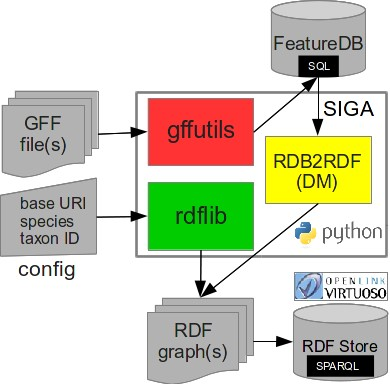
\includegraphics[scale=0.9]{FigureA1.jpg} %figure added
\caption{\hl{SIGA.py software architecture.}} 
\label{FigureA1}
\end{figure} 

\section{Supplementary~Tables}
%All appendix sections must be cited in the main text. In the appendixes, Figures, Tables, etc. should be labeled starting with `A', e.g.,~Figure A1, Figure A2, etc. 
\vspace{-3mm}

\begin{table}[H]
\centering
%\captionsetup{width=0.95\linewidth,skip=8pt}
\caption{\textbf{\hl{List of RESTful APIs} %MDPI: is the bold necessary? No, can be removed
 of pbg-ld {generated} with the help of  grlc service. These REST APIs can be accessed with the following locations: \url{http://DomainLocation/api/APIendpoints?variables}.}}
\label{SP:Table1}
\scalebox{.78}[.78]{\begin{tabular}{m{1.2cm}<{\raggedright}m{3cm}<{\raggedright}m{3.5cm}<{\raggedright}m{4.5cm}<{\raggedright}m{3cm}<{\raggedright}m{1.8cm}<{\raggedright}}
\toprule
\textbf{Number} & \textbf{Endpoint (Path)} & \textbf{Description} & \textbf{Input Variables} & \textbf{Response fields} &  \textbf{Exemplary Link on localhost:8080}  \\
%\midrule
\midrule
1. & /countFeatures & Count genomic features given a (input) genome graph. & \makecell[l]{graph: Genome graph URI, \\
endpoint: Sparql endpoint} & \makecell[l]{feature{\_}id, \\  feature{\_}uri, \\ feature} &  \href{http://localhost:8080/api/candYgene/queries/countFeatures?graph=http://plants.ensembl.org/Solanum_lycopersicum}{\hl{[link]} %MDPI: should it be original link or please complete by detailed website link? These urls in this manuscript should be used. They will resolve to the correct page, only if the presetned software is isnstalled by the reader (as this sis the core of the paper). So, please do not modify these.
}  \\ %[1cm]

2.& /getGeneAnnotations & Get annotations from SGN given a (input) sgn{\_} and gene{\_}id. & \makecell[l]{geneid: Solyc id of the gene \\ endpoint: Sparql endpoint} &  \makecell[l]{gene{\_}uri, \\ gene{\_}annotations} &\href{http://localhost:8080/api/candYgene/queries/countFeatures?geneid=Solyc01g00500*}{[link]}  \\ %[1cm]

3. & /getGenesInQTL & Get genes contained in a QTL, given (input) qtl{\_}id & \makecell[l] {qtlid:QTM id of the QTL \\ endpoint: Sparql endpoint} & gene{\_}id, gene{\_}uri & \href{http://localhost:8080/api/candYgene/queries/countFeatures?qtlid=QTL:3859326_3_2}{[link]}   \\ %[1cm]

4. & /getQTLinArticle & Get QTLs in an article, given (input) pmc{\_}id.& \makecell[l]{ pmcid: Pubmed Central ID \\ endpoint: Sparql endpoint} & \makecell[l]{qtl{\_}id, \\ qtl{\_}uri}  & \href{http://localhost:8080/api/candYgene/queries/countFeatures?pmcid=PMC4321030}{[link]}  \\ %[1cm]

5. & /getQTLs & Get QTLs associated with a trait, given (input) trait{\_}id.& \makecell[l]{traitid: TO/SPTO id  \\ endpoint: Sparql endpoint} &  \makecell[l]{qtl{\_}id,qtl{\_}uri}  & \href{http://localhost:8080/api/candYgene/queries/countFeatures?traitid=SP:0000201}{[link]}  \\ %[1cm]

6. &/ getTraitIds & Get trait\_ids given a (input) trait name. & \makecell[l]{traitname: The name of the trait \\ endpoint: Sparql endpoint} & \makecell[l]{trait{\_}id, \\ trait{\_}term, \\ trait{\_}uri}  & \href{http://localhost:8080/api/candYgene/queries/countFeatures?traitname=Tuber\%20AND\%20Shape}{[link]}  \\ [1cm]

7. & /summarizeQTLs & Summarize QTLs extracted from articles, given (input) pmc{\_}id & \makecell[l]{ pmcid: Pubmed Central ID \\ endpoint: Sparql endpoint} & \makecell[l]{qtl{\_}id, \\ associated{\_}trait, \\ chromosomal{\_}location}  & \href{http://localhost:8080/api/candYgene/queries/countFeatures?pmcid=PMC4321030}{[link]}  \\ %[1cm]
\bottomrule
\end{tabular}}
\end{table}


%%%%%%%%%%%%%%%%%%%%%%%%%%%%%%%%%%%%%%%%%%
% Citations and References in Supplementary files are permitted provided that they also appear in the reference list here. 

%=====================================
% References, variant A: internal bibliography
%=====================================

%\begin{thebibliography}{999}
% Reference 1
%\bibitem[Author1(year)]{ref-journal}
%Author1, T. The title of the cited article. {\em Journal Abbreviation} {\bf 2008}, {\em 10}, 142--149.
% Reference 2
%\bibitem[Author2(year)]{ref-book}
%Author2, L. The title of the cited contribution. In {\em The Book Title}; Editor1, F., Editor2, A., Eds.; Publishing House: City, Country, 2007; pp. 32--58.
%\end{thebibliography}


% The following MDPI journals use author-date citation: Arts, Econometrics, Economies, Genealogy, Humanities, IJFS, JRFM, Laws, Religions, Risks, Social Sciences. For those journals, please follow the formatting guidelines on http://www.mdpi.com/authors/references
% To cite two works by the same author: \citeauthor{ref-journal-1a} (\citeyear{ref-journal-1a}, \citeyear{ref-journal-1b}). This produces: Whittaker (1967, 1975)
% To cite two works by the same author with specific pages: \citeauthor{ref-journal-3a} (\citeyear{ref-journal-3a}, p. 328; \citeyear{ref-journal-3b}, p.475). This produces: Wong (1999, p. 328; 2000, p. 475)



%\newpage 
%=====================================
 %References, variant B: external bibliography
%=====================================

\reftitle{References}

% \begin{thebibliography}{999}
% %\providecommand{\natexlab}[1]{#1}

% \bibitem[Consortium \em{et~al.}(2012)Consortium et~al.]{tomato2012tomato}
% Tomato Genome Consortium.
% \newblock The tomato genome sequence provides insights into fleshy fruit
%   evolution.
% \newblock {\em Nature} {\bf 2012}, {\em 485},~635.

% \bibitem[Consortium \em{et~al.}(2011)Consortium et~al.]{potato2011genome}
% Potato Genome Sequencing Consortium.
% \newblock Genome sequence and analysis of the tuber crop potato.
% \newblock {\em Nature} {\bf 2011}, {\em 475},~189.

% \bibitem[Wang \em{et~al.}(2011)Wang, Wang, Wang, Sun, Wu, Liu, Bai, Mun,
%   Bancroft, Cheng, et~al.]{wang2011genome}
% Wang, X.; Wang, H.; Wang, J.; Sun, R.; Wu, J.; Liu, S.; Bai, Y.; Mun, J.H.;
%   Bancroft, I.; Cheng, F.; et al.
% \newblock The~genome of the mesopolyploid crop species Brassica rapa.
% \newblock {\em Nat. Genet.} {\bf 2011}, {\em 43},~1035.

% \bibitem[Huang \em{et~al.}(2009)Huang, Li, Zhang, Li, Gu, Fan, Lucas, Wang,
%   Xie, Ni, et~al.]{huang2009genome}
% Huang, S.; Li, R.; Zhang, Z.; Li, L.; Gu, X.; Fan, W.; Lucas, W.J.; Wang, X.;
%   Xie, B.; Ni, P.; et al.
% \newblock The genome of the cucumber, \emph{Cucumis sativus} L.
% \newblock {\em Nat. Genet.} {\bf 2009}, {\em 41},~1275.

% \bibitem[Chibon \em{et~al.}(2012)Chibon, Schoof, Visser, and
%   Finkers]{chibon2012marker2sequence}
% Chibon, P.Y.; Schoof, H.; Visser, R.G.; Finkers, R.
% \newblock Marker2sequence, mine your QTL regions for candidate genes.
% \newblock {\em Bioinformatics} {\bf 2012}, {\em 28},~1921--1922.

% \bibitem[Astola \em{et~al.}(2014)Astola, Stigter, van Dijk, van Daelen, and
%   Molenaar]{astola2014inferring}
% Astola, L.; Stigter, H.; van Dijk, A.D.; van Daelen, R.; Molenaar, J.
% \newblock Inferring the gene network underlying the branching of tomato
%   inflorescence.
% \newblock {\em PLoS ONE} {\bf 2014}, {\em 9},~e89689.

% \bibitem[Shinozuka \em{et~al.}(2012)Shinozuka, Cogan, Spangenberg, and
%   Forster]{shinozuka2012quantitative}
% Shinozuka, H.; Cogan, N.O.; Spangenberg, G.C.; Forster, J.W.
% \newblock Quantitative Trait Locus (QTL) meta-analysis and comparative genomics
%   for candidate gene prediction in perennial ryegrass (\emph{Lolium perenne} L.).
% \newblock {\em BMC~Genet.} {\bf 2012}, {\em 13},~101.

% \bibitem[Durinx \em{et~al.}(2016)Durinx, McEntyre, Appel, Apweiler, Barlow,
%   Blomberg, Cook, Gasteiger, Kim, Lopez, et~al.]{durinx2016identifying}
% Durinx, C.; McEntyre, J.; Appel, R.; Apweiler, R.; Barlow, M.; Blomberg, N.;
%   Cook, C.; Gasteiger, E.; Kim, J.H.; Lopez, R.; et al.
% \newblock Identifying ELIXIR core data resources.
% \newblock {\em F1000Research} {\bf 2016}, {\em \hl{1-17} %MDPI: please add page.Done.

% \bibitem[Harrison \em{et~al.}(2018)Harrison, Alako, Amid,
%   Cerde{\~n}o-T{\'a}rraga, Cleland, Holt, Hussein, Jayathilaka, Kay, Keane,
%   et~al.]{harrison2018european}
% Harrison, P.W.; Alako, B.; Amid, C.; Cerde{\~n}o-T{\'a}rraga, A.; Cleland, I.;
%   Holt, S.; Hussein, A.; Jayathilaka, S.; Kay, S.; Keane, T.; et al.
% \newblock The European Nucleotide Archive in 2018.
% \newblock {\em Nucleic Acids Res.} {\bf 2018}, {\em 47},~D84--D88.

% \bibitem[Bolser \em{et~al.}(2017)Bolser, Staines, Perry, and
%   Kersey]{bolser2017ensembl}
% Bolser, D.M.; Staines, D.M.; Perry, E.; Kersey, P.J.
% \newblock Ensembl plants: Integrating tools for visualizing, mining, and
%   analyzing plant genomic data. In {\em Plant Genomics Databases}; Springer:  \hl{Berlin/Heidelberg, Germany,} %newly added information, please confirm | OK
%   2017; pp. 1--31.

% \bibitem[Pundir \em{et~al.}(2017)Pundir, Martin, and
%   O’Donovan]{pundir2017uniprot}
% Pundir, S.; Martin, M.J.; O’Donovan, C.
% \newblock UniProt protein knowledgebase. In {\em Protein Bioinformatics};
%   Springer:  \hl{Berlin/Heidelberg, Germany,} %newly added information, please confirm | OK
%   2017; pp. 41--55.

% \bibitem[Mueller \em{et~al.}(2005)Mueller, Solow, Taylor, Skwarecki, Buels,
%   Binns, Lin, Wright, Ahrens, Wang, et~al.]{mueller2005sol}
% Mueller, L.A.; Solow, T.H.; Taylor, N.; Skwarecki, B.; Buels, R.; Binns, J.;
%   Lin, C.; Wright, M.H.; Ahrens, R.; Wang, Y.; et al.
% \newblock The SOL Genomics Network. A comparative resource for Solanaceae
%   biology and beyond.
% \newblock {\em Plant Physiol.} {\bf 2005}, {\em 138},~1310--1317.

% \bibitem[Arnold~Kuzniar()]{Kuzniarpbgld}
% Arnold~Kuzniar, G.S.
% \newblock Solanacea Linked Data Platform.
% \newblock Available online: \url{http://pbg-ld.candygene-nlesc.surf-hosted.nl/fct/}
% \newblock  (accessed on 1 July 2012).

% \bibitem[Berners-Lee(2006)]{Berners-Lee2006}
% Berners-Lee, T.
% \newblock {Linked Data}. 2006.
% \newblock Available online: \url{https://www.w3.org/DesignIssues/LinkedData.html}
% \newblock (accessed on 1 July 2012).

% \bibitem[Wilkinson \em{et~al.}(2016)Wilkinson, Dumontier, Aalbersberg,
%   Appleton, Axton, Baak, Blomberg, Boiten, da~Silva~Santos, Bourne,
%   et~al.]{wilkinson2016fair}
% Wilkinson, M.D.; Dumontier, M.; Aalbersberg, I.J.; Appleton, G.; Axton, M.;
%   Baak, A.; Blomberg, N.; Boiten,~J.W.; da~Silva~Santos, L.B.; Bourne, P.E.;
%   et al.
% \newblock The FAIR Guiding Principles for scientific data management and
%   stewardship.
% \newblock {\em Sci. Data} {\bf 2016}, {\em 3}, 1--9.

% \bibitem[SPT()]{SPTO}
% SPTO: Solanaceae Phenotype Ontology.
% \newblock
%  Available online:  \url{http://bioportal.bioontology.org/ontologies/SPTO?p=classes&conceptid=root}
% \newblock (accessed on 1 July 2012).

% \bibitem[Shrestha \em{et~al.}(2012)Shrestha, Matteis, Skofic, Portugal,
%   McLaren, Hyman, and Arnaud]{CO}
% Shrestha, R.; Matteis, L.; Skofic, M.; Portugal, A.; McLaren, G.; Hyman, G.;
%   Arnaud, E.
% \newblock {Bridging~the phenotypic and genetic data useful for integrated
%   breeding through a data annotation using the Crop Ontology developed by the
%   crop communities of practice}.
% \newblock {\em Front. Physiol.} {\bf 2012}, {\em 3},~326, doi:10.3389/fphys.2012.00326.

% \bibitem[Cooper \em{et~al.}(2013)Cooper, Walls, Elser, Gandolfo, Stevenson,
%   Smith, Preece, Athreya, Mungall, Rensing, Hiss, Lang, Reski, Berardini, Li,
%   Huala, Schaeffer, Menda, Arnaud, Shrestha, Yamazaki, and
%   Jaiswal]{doi:10.1093/pcp/pcs163}
% Cooper, L.; Walls, R.L.; Elser, J.; Gandolfo, M.A.; Stevenson, D.W.; Smith, B.;
%   Preece, J.; Athreya, B.; Mungall,~C.J.; Rensing, S.; et al.
% \newblock {The Plant Ontology as a Tool for Comparative Plant Anatomy and
%   Genomic Analyses}.
% \newblock {\em Plant Cell Physiol.} {\bf 2013}, {\em 54},~e1, doi:10.1093/pcp/pcs163.

% \bibitem[Walls \em{et~al.}(2012)Walls, Athreya, Cooper, Elser, Gandolfo,
%   Jaiswal, Mungall, Preece, Rensing, Smith, and Stevenson]{Walls2012}
% Walls, R.L.; Athreya, B.; Cooper, L.; Elser, J.; Gandolfo, M.A.; Jaiswal, P.;
%   Mungall, C.J.; Preece, J.; Rensing,~S.; Smith, B.; et al.
% \newblock {Ontologies as integrative tools for plant science.}
% \newblock {\em Am. J. Bot.} {\bf 2012}, {\em 99},~1263--1275, doi:10.3732/ajb.1200222.

% \bibitem[TO()]{TO}
% TO: Trait Ontology.
% \newblock
%  Available online:  \url{https://raw.githubusercontent.com/Planteome/plant-trait-ontology/master/to.owl}
% \newblock  (accessed on 1 July 2012).

% \bibitem[Consortium(2017)]{GOontology}
% The Gene Ontology Consortium.
% \newblock Expansion of the Gene Ontology knowledgebase and resources.
% \newblock {\em Nucleic~Acids Res.} {\bf 2017}, {\em 45},~D331--D338.

% \bibitem[Eilbeck \em{et~al.}(2005)Eilbeck, Lewis, Mungall, Yandell, Stein,
%   Durbin, and Ashburner]{Eilbeck2005}
% Eilbeck, K.; Lewis, S.E.; Mungall, C.J.; Yandell, M.; Stein, L.; Durbin, R.;
%   Ashburner, M.
% \newblock {The~Sequence Ontology: A tool for the unification of genome
%   annotations}.
% \newblock {\em Genome Biol.} {\bf 2005}, {\em 6},~R44, doi:10.1186/gb-2005-6-5-r44.

% \bibitem[FAL()]{FALDO}
% {FALDO Ontology}.
% \newblock Available online:  \url{http://biohackathon.org/resource/faldo.rdf}.
% \newblock  (accessed on 1 July 2012).

% \bibitem[Hastings \em{et~al.}(2013)Hastings, de~Matos, Dekker, Ennis, Harsha,
%   Kale, Muthukrishnan, Owen, Turner, Williams, and Steinbeck]{Hastings2013}
% Hastings, J.; de~Matos, P.; Dekker, A.; Ennis, M.; Harsha, B.; Kale, N.;
%   Muthukrishnan, V.; Owen, G.; Turner,~S.; Williams, M.; et al.
% \newblock {The ChEBI reference database and ontology for biologically relevant
%   chemistry: Enhancements for 2013.}
% \newblock {\em Nucleic Acids Res.} {\bf 2013}, {\em 41},~D456--D463, doi:10.1093/nar/gks1146.

% \bibitem[Garcia-Hernandez \em{et~al.}(2002)Garcia-Hernandez, Berardini, Chen,
%   Crist, Doyle, Huala, Knee, Lambrecht, Miller, Mueller,
%   et~al.]{garcia2002tair}
% Garcia-Hernandez, M.; Berardini, T.; Chen, G.; Crist, D.; Doyle, A.; Huala, E.;
%   Knee, E.; Lambrecht, M.; Miller,~N.; Mueller, L.A.; et al.
% \newblock TAIR: A resource for integrated Arabidopsis data.
% \newblock {\em Funct. Integr. Genom.} {\bf 2002}, {\em
%   2},~239--253.

% \bibitem[Nakaya \em{et~al.}(2017)Nakaya, Ichihara, Asamizu, Shirasawa,
%   Nakamura, Tabata, and Hirakawa]{nakaya2017plant}
% Nakaya, A.; Ichihara, H.; Asamizu, E.; Shirasawa, S.; Nakamura, Y.; Tabata, S.;
%   Hirakawa, H.
% \newblock Plant genome database japan (PGDBj). In {\em Plant Genomics
%   Databases}; Springer:  \hl{Berlin/Heidelberg, Germany,} %newly added information, please confirm OK
%  2017; pp. 45--77.

% \bibitem[Cooper \em{et~al.}(2018)Cooper, Meier, Laporte, Elser, Mungall, Sinn,
%   Cavaliere, Carbon, Dunn, Smith, Qu, Preece, Zhang, Todorovic, Gkoutos,
%   Doonan, Stevenson, Arnaud, and Jaiswal]{Cooper2018}
% Cooper, L.; Meier, A.; Laporte, M.A.; Elser, J.L.; Mungall, C.; Sinn, B.T.;
%   Cavaliere, D.; Carbon, S.; Dunn, N.A.; Smith, B.; et al.
% \newblock {The Planteome database: An integrated resource for reference
%   ontologies, plant genomics and phenomics.}
% \newblock {\em Nucleic Acids Res.} {\bf 2018}, {\em 46},~D1168--D1180, doi:10.1093/nar/gkx1152.

% \bibitem[Kuzniar(2018)]{kuzniar_arnold_2018_1458169}
% Kuzniar, A.
% \newblock {\em pbg-ld: Linked Data Platform for Plant Breeding \& Genomics};  \hl{2018;} %MDPI: please add oublisher and location. This is a data repository. The DOI will be sufficient
%  doi:10.5281/zenodo.1458169.

% \bibitem[Mero{\~{n}}o-Pe{\~{n}}uela and Hoekstra(2016)]{Merono-Penuela2016}
% Mero{\~{n}}o-Pe{\~{n}}uela, A.; Hoekstra, R.
% \newblock {\em grlc Makes GitHub Taste Like Linked Data APIs}.
% \newblock  The Semantic Web, Sack,~H., Rizzo, G., Steinmetz, N.,
%   Mladeni{\'{c}}, D., Auer, S., Lange, C., Eds.; Springer International
%   Publishing: Cham, Switzerland, 2016; pp. 342--353.

% \bibitem[Consortium(2015)]{europe2015europe}
% Consortium, E.P.
% \newblock Europe PMC: A full-text literature database for the life sciences and
%   platform for innovation.
% \newblock {\em Nucleic Acids Res.} {\bf 2015}, {\em 43},~D1042--D1048.

% \bibitem[GFF()]{GFF3}
% Generic Feature Format Version 3 (GFF3).
% \newblock Available online: \url{http://www.sequenceontology.org/resources/gff3.html}
% \newblock  (accessed on 1 July 2020).

% \bibitem[Singh \em{et~al.}(2018)Singh, Kuzniar, van Mulligen, Gavai, Bachem,
%   Visser, and Finkers]{singh2018qtltableminer++}
% Singh, G.; Kuzniar, A.; van Mulligen, E.M.; Gavai, A.; Bachem, C.W.; Visser,
%   R.G.; Finkers, R.
% \newblock QTLTableMiner++: Semantic mining of QTL tables in scientific
%   articles.
% \newblock {\em BMC Bioinform.} {\bf 2018}, {\em 19},~183.

% \bibitem[Singh and Kuzniar(2019)]{singh_gurnoor_2019_1193640}
% Singh, G.; Kuzniar, A.
% \newblock {QTLTableMiner++:(v1.1.0)}.  2019.
% \newblock Available online:  \url{https://doi.org/10.5281/zenodo.1193640}
% \newblock (accessed on 1 July 2020).
%  % doi:{\changeurlcolor{black}\href{https://doi.org/10.5281/zenodo.1193640}{\detokenize{10.5281/zenodo.1193640}}}.

% \bibitem[Kuzniar(2017)]{Kuzniar2017}
% Kuzniar, A.
% \newblock {SIGA.py, A Light-Weight Command-Line Tool to Generate Semantically
%   Interoperable Genome Annotations from GFF Files.} 2017.
% \newblock Available online:  \url{https://zenodo.org/record/1076438}
% \newblock (accessed on \mbox{1 July 2020}).
%  % doi:{\changeurlcolor{black}\href{https://doi.org/10.5281/ZENODO.1076438}{\detokenize{10.5281/ZENODO.1076438}}}.

% \bibitem[Lyo()]{LyocITAG2.4}
% {Solanum{\_}lycopersicum(ITAG2.4)}.
% \newblock
%   Available online:  \url{ftp://ftp.solgenomics.net/genomes/Solanum_lycopersicum/annotation/ITAG2.4_release/}
% \newblock (accessed on 1 July 2020).

% \bibitem[Pen()]{PennITAG2.4}
% {Solanum{\_}pennellii(ITAG2.4)}.
% \newblock Available online:  \url{ftp://ftp.solgenomics.net/genomes/Solanum_pennellii}
% \newblock (accessed on 1 July 2020).

% \bibitem[PGS()]{PGSCDM}
% {Solanum{\_}pennellii(ITAG2.4)}.
% \newblock Available online:  \url{ftp://ftp.solgenomics.net/genomes/Solanum_tuberosum/}
% \newblock (accessed on 1 July 2020).

% \bibitem[Ens({\natexlab{a}})]{EnsemblPlantSolanumlycopersicum}
% {EnsemblPlant:Solanum Lycopersicum}.
% \newblock Available online:  \url{http://plants.ensembl.org/Solanum_lycopersicum}
% \newblock (accessed on 1 July 2020).

% \bibitem[Ens({\natexlab{b}})]{EnsemblPlantSolanumtuberosum}
% {EnsemblPlant:Solanum Tuberosum}.
% \newblock Available online:  \url{http://plants.ensembl.org/Solanum_tuberosum}
% \newblock (accessed on 1 July 2020).

% \bibitem[Uni({\natexlab{a}})]{UniprotSL}
% {Uniprot: Solanum Lycopersicum}.
% \newblock Available online:   \url{http://www.uniprot.org/proteomes/Solanum_lycopersicum}
% \newblock (accessed on 1 July 2020).

% \bibitem[Uni({\natexlab{b}})]{UniprotST}
% {Uniprot: Solanum Tuberosum}.
% \newblock Available online:  \url{http://www.uniprot.org/proteomes/Solanum_tuberosum}
% \newblock (accessed on 1 July 2020).

% \bibitem[Uni({\natexlab{c}})]{UniprotRDFcore}
% {Uniprot RDF Core Ontology}.
% \newblock Available online:  \url{https://www.uniprot.org/core/}
% \newblock (accessed on 1 July 2020).

% \bibitem[SIO()]{SIO}
% {Semanticscience Integrated Ontology.}
% \newblock Available online:  \url{http://semanticscience.org/ontology/sio.owl}
% \newblock (accessed on 1 July 2020).

% \bibitem[RO()]{RO}
% {RO: Relation Ontology}.
% \newblock Available online:  \url{http://purl.obolibrary.org/obo/ro.owl}
% \newblock (accessed on 1 July 2020).

% \bibitem[Boettiger(2015)]{boettiger2015introduction}
% Boettiger, C.
% \newblock An introduction to Docker for reproducible research.
% \newblock {\em ACM SIGOPS Oper. Syst. Rev.} {\bf 2015}, {\em
%   49},~71--79.

% \bibitem[Ansible()]{ansible}
% Ansible, R.H.
% \newblock Ansible Is Simple IT Automation.
% \newblock Available online:  \url{https://www.ansible.com/}
% \newblock (accessed on 1 July 2020).

% \bibitem[Haggard \em{et~al.}(2015)Haggard, Johnson, and
%   Clair]{haggard2015multiple}
% Haggard, J.E.; Johnson, E.B.; Clair, D.A.S.
% \newblock Multiple QTL for horticultural traits and quantitative resistance to
%   Phytophthora infestans linked on Solanum habrochaites chromosome 11.
% \newblock {\em G3  Genes Genomes Genet.} {\bf 2015}, {\em 5},~219--233.

% \bibitem[Kluyver \em{et~al.}(2016)Kluyver, Ragan-Kelley, P{\'e}rez, Granger,
%   Bussonnier, Frederic, Kelley, Hamrick, Grout, Corlay,
%   et~al.]{kluyver2016jupyter}
% Kluyver, T.; Ragan-Kelley, B.; P{\'e}rez, F.; Granger, B.E.; Bussonnier, M.;
%   Frederic, J.; Kelley, K.; Hamrick, J.B.; Grout, J.; Corlay, S.; et al.
% \newblock Jupyter Notebooks-a publishing format for reproducible computational
%   workflows.
% \newblock  In \emph{IOS Press ebook}; \hl{ 2016;} %MDPI: please add publisher and location. The DOI is: 10.3233/978-1-61499-649-1-87  ; hope that I modified the bibliography correctly
%  pp. 87--90.

% \bibitem[Not()]{Noteboook:example1}
% A Jupyter Notebook to Compare QTLs for Tomato Fruit Shape and Potato Tuber
%   Shape.
% \newblock
%  Available~online:  \url{https://github.com/candYgene/notebooks/blob/master/example_1/QTL_fruit_tuber_shape_gene_loss.ipynb}
% \newblock (accessed on 1 July 2020).

% \bibitem[Wu \em{et~al.}(2018)Wu, Zhang, Keyhaninejad, et~al.]{wu2018common}
% Wu, S.; Zhang, B.; Keyhaninejad, N.; Rodríguez, G.R.; Kim, H.J.; Chakrabarti, M.; Illa-Berenguer, E.; Taitano,~N.K.; Gonzalo, M.J.; Díaz, A.; et al.
% \newblock A common genetic mechanism underlies morphological diversity in
%   fruits and other plant organs.
% \newblock {\em Nat. Commun.} {\bf 2018}, {\em 9},~4734.

% \bibitem[Ballester \em{et~al.}(2016)Ballester, Tikunov, Molthoff, Grandillo,
%   Viquez-Zamora, de~Vos, de~Maagd, van Heusden, and
%   Bovy]{ballester2016identification}
% Ballester, A.; Tikunov, Y.; Molthoff, J.; Grandillo, S.; Viquez-Zamora, M.;
%   de~Vos, R.; de~Maagd, R.; van~Heusden,~S.; Bovy, A.
% \newblock Identification of Loci Affecting Accumulation of Secondary
%   Metabolites in Tomato Fruit of a Solanum lycopersicum X Solanum chmielewskii
%   Introgression Line Population.
% \newblock {\em \mbox{Front. Plant Sci.}} {\bf 2016}, {\em 7},~1428.

% \bibitem[Shulaev \em{et~al.}(1997)Shulaev, Silverman, and
%   Raskin]{shulaev1997airborne}
% Shulaev, V.; Silverman, P.; Raskin, I.
% \newblock Airborne signalling by methyl salicylate in plant pathogen
%   resistance.
% \newblock {\em Nature} {\bf 1997}, {\em 385},~718.

% \bibitem[Luengwilai \em{et~al.}(2010)Luengwilai, Fiehn, and
%   Beckles]{luengwilai2010comparison}
% Luengwilai, K.; Fiehn, O.E.; Beckles, D.M.
% \newblock Comparison of leaf and fruit metabolism in two tomato (\emph{Solanum
%   lycopersicum} L.) genotypes varying in total soluble solids.
% \newblock {\em J. Agric. Food Chem.} {\bf 2010}, {\em
%   58},~11790--11800.

% \bibitem[Di~Mascio \em{et~al.}(1989)Di~Mascio, Kaiser, and
%   Sies]{di1989lycopene}
% Di~Mascio, P.; Kaiser, S.; Sies, H.
% \newblock Lycopene as the most efficient biological carotenoid singlet oxygen
%   quencher.
% \newblock {\em Arch. Biochem. Biophys.} {\bf 1989}, {\em
%   274},~532--538.

% \bibitem[Falara \em{et~al.}(2011)Falara, Akhtar, Nguyen, Spyropoulou, Bleeker,
%   Schauvinhold, Matsuba, Bonini, Schilmiller, Last, et~al.]{falara2011tomato}
% Falara, V.; Akhtar, T.A.; Nguyen, T.T.; Spyropoulou, E.A.; Bleeker, P.M.;
%   Schauvinhold, I.; Matsuba, Y.; Bonini,~M.E.; Schilmiller, A.L.; Last, R.L.;
%   et al.
% \newblock The tomato terpene synthase gene family.
% \newblock {\em Plant Physiol.} {\bf 2011}, {\em 157},~770--789.

% \bibitem[Warwick~Vesztrocy \em{et~al.}(2018)Warwick~Vesztrocy, Dessimoz, and
%   Redestig]{warwick2018prioritising}
% Warwick~Vesztrocy, A.; Dessimoz, C.; Redestig, H.
% \newblock Prioritising candidate genes causing QTL using hierarchical
%   orthologous groups.
% \newblock {\em Bioinformatics} {\bf 2018}, {\em 34},~i612--i619.

% \bibitem[Lin \em{et~al.}(2019)Lin, Fan, and Rhee]{lin2019qtg}
% Lin, F.; Fan, J.; Rhee, S.Y.
% \newblock QTG-Finder: A machine-learning based algorithm to prioritize causal
%   genes of quantitative trait loci in Arabidopsis and rice.
% \newblock {\em G3: GENES, GENOMES, GENETICS} {\bf 2019}, {\em 9} \hl{3129-3138.} %MDPI: PLEASE add volume. Modified from BioRVX to published version: https://doi.org/10.1534/g3.119.400319


% \bibitem[Schneider \em{et~al.}(2007)Schneider, Dessimoz, and
%   Gonnet]{schneider2007oma}
% Schneider, A.; Dessimoz, C.; Gonnet, G.H.
% \newblock OMA Browser—exploring orthologous relations across 352 complete
%   genomes.
% \newblock {\em Bioinformatics} {\bf 2007}, {\em 23},~2180--2182.

% \bibitem[Not()]{Noteboook:example2}
% \hl{A Jupyter Notebook to Compare QTLs for Tomato Fruit Shape and Potato Tuber
%   Shape.} %The titles of ref.59 and ref.49 are the same, please recheck if they are duplicated. No, they are different; they resolve to different pieces of supporting data in the github repository.
% \newblock Available online:  
%   \url{https://github.com/candYgene/notebooks/tree/master/biological\%20usecase2}
% \newblock (accessed on 1 July 2020).

% \bibitem[Fridman \em{et~al.}(2002)Fridman, Liu, Carmel-Goren, Gur, Shoresh,
%   Pleban, Eshed, and Zamir]{fridman2002two}
% Fridman, E.; Liu, Y.; Carmel-Goren, L.; Gur, A.; Shoresh, M.; Pleban, T.;
%   Eshed, Y.; Zamir, D.
% \newblock Two tightly linked QTLs modify tomato sugar content via different
%   physiological pathways.
% \newblock {\em Mol. Genet. Genom.} {\bf 2002}, {\em
%   266},~821--826.

% \bibitem[Bouvier \em{et~al.}(2000)Bouvier, D’Harlingue, Backhaus, Kumagai,
%   and Camara]{bouvier2000identification}
% Bouvier, F.; D’Harlingue, A.; Backhaus, R.A.; Kumagai, M.H.; Camara, B.
% \newblock Identification of neoxanthin synthase as a carotenoid cyclase
%   paralog.
% \newblock {\em Eur. J. Biochem.} {\bf 2000}, {\em
%   267},~6346--6352.

% \bibitem[Tadmor \em{et~al.}(2002)Tadmor, Fridman, Gur, Larkov, Lastochkin,
%   Ravid, Zamir, and Lewinsohn]{tadmor2002identification}
% Tadmor, Y.; Fridman, E.; Gur, A.; Larkov, O.; Lastochkin, E.; Ravid, U.; Zamir,
%   D.; Lewinsohn, E.
% \newblock Identification of malodorous, a wild species allele affecting tomato
%   aroma that was selected against during domestication.
% \newblock {\em J. Agric. Food Chem.} {\bf 2002}, {\em
%   50},~2005--2009.

% \bibitem[Marti \em{et~al.}(2016)Marti, Rosello, and
%   Cebolla-Cornejo]{marti2016tomato}
% Marti, R.; Rosello, S.; Cebolla-Cornejo, J.
% \newblock Tomato as a source of carotenoids and polyphenols targeted to cancer
%   prevention.
% \newblock {\em Cancers} {\bf 2016}, {\em 8},~58.

% \bibitem[Giuliano(2014)]{giuliano2014plant}
% Giuliano, G.
% \newblock Plant carotenoids: Genomics meets multi-gene engineering.
% \newblock {\em Curr. Opin. Plant Biol.} {\bf 2014}, {\em
%   19},~111--117.

% \bibitem[Shi \em{et~al.}(2004)Shi, Kakuda, and Yeung]{shi2004antioxidative}
% Shi, J.; Kakuda, Y.; Yeung, D.
% \newblock Antioxidative properties of lycopene and other carotenoids from
%   tomatoes: Synergistic effects.
% \newblock {\em Biofactors} {\bf 2004}, {\em 21},~203--210.

% \bibitem[Cunningham \em{et~al.}(1996)Cunningham, Pogson, Sun, McDonald,
%   DellaPenna, and Gantt]{cunningham1996functional}
% Cunningham, F.X.; Pogson, B.; Sun, Z.; McDonald, K.A.; DellaPenna, D.; Gantt,
%   E.
% \newblock Functional analysis of the beta and epsilon lycopene cyclase enzymes
%   of Arabidopsis reveals a mechanism for control of cyclic carotenoid
%   formation.
% \newblock {\em  Plant Cell} {\bf 1996}, {\em 8},~1613--1626.

% \bibitem[Rousseaux \em{et~al.}(2005)Rousseaux, Jones, Adams, Chetelat, Bennett,
%   and Powell]{rousseaux2005qtl}
% Rousseaux, M.C.; Jones, C.M.; Adams, D.; Chetelat, R.; Bennett, A.; Powell, A.
% \newblock QTL analysis of fruit antioxidants in tomato using Lycopersicon
%   pennellii introgression lines.
% \newblock {\em Theor. Appl. Genet.} {\bf 2005}, {\em
%   111},~1396--1408.

% \bibitem[Tieman \em{et~al.}(2007)Tieman, Loucas, Kim, Clark, and
%   Klee]{tieman2007tomato}
% Tieman, D.M.; Loucas, H.M.; Kim, J.Y.; Clark, D.G.; Klee, H.J.
% \newblock Tomato phenylacetaldehyde reductases catalyze the last step in the
%   synthesis of the aroma volatile 2-phenylethanol.
% \newblock {\em Phytochemistry} {\bf 2007}, {\em 68},~2660--2669.

% \bibitem[Zhang \em{et~al.}(2015)Zhang, Zhao, Xu, Liang, Chang, Yan, Li, Liang,
%   and Zou]{zhang2015genome}
% Zhang, J.; Zhao, J.; Xu, Y.; Liang, J.; Chang, P.; Yan, F.; Li, M.; Liang, Y.;
%   Zou, Z.
% \newblock Genome-wide association mapping for tomato volatiles positively
%   contributing to tomato flavor.
% \newblock {\em Front. Plant Sci.} {\bf 2015}, {\em 6},~1042.

% \bibitem[Socaci \em{et~al.}(2014)Socaci, Socaciu, Mure{\c{s}}an,
%   F{\u{a}}rca{\c{s}}, Tofan{\u{a}}, Vica{\c{s}}, and
%   Pintea]{socaci2014chemometric}
% Socaci, S.A.; Socaciu, C.; Mure{\c{s}}an, C.; F{\u{a}}rca{\c{s}}, A.;
%   Tofan{\u{a}}, M.; Vica{\c{s}}, S.; Pintea, A.
% \newblock Chemometric discrimination of different tomato cultivars based on
%   their volatile fingerprint in relation to lycopene and total phenolics
%   content.
% \newblock {\em Phytochem. Anal.} {\bf 2014}, {\em 25},~161--169.

% \bibitem[Rambla \em{et~al.}(2016)Rambla, Medina, Fernandez-del Carmen,
%   Barrantes, Grandillo, Cammareri, Lopez-Casado, Rodrigo, Alonso,
%   Garcia-Martinez, et~al.]{rambla2016identification}
% Rambla, J.L.; Medina, A.; Fernandez-del Carmen, A.; Barrantes, W.; Grandillo,
%   S.; Cammareri, M.; Lopez-Casado, G.; Rodrigo, G.; Alonso, A.;
%   Garcia-Martinez, S.; et al.
% \newblock Identification, introgression, and validation of fruit volatile QTLs
%   from a red-fruited wild tomato species.
% \newblock {\em J. Exp. Bot.} {\bf 2016}, {\em 68},~429--442.

% \bibitem[Hassani-Pak and Rawlings(2017)]{hassani2017knowledge}
% Hassani-Pak, K.; Rawlings, C.
% \newblock Knowledge discovery in biological databases for revealing candidate
%   genes linked to complex phenotypes.
% \newblock {\em J. Integr. Bioinform.} {\bf 2017}, {\em \hl{14},~1-9 %MDPI: PLEASE add page. Added
% }.

% \bibitem[Kne()]{Knetresources}
% Available Resources of the KNETMiner Tool.~Available online: \url{https://knetminer.com/resources}
% \newblock  (accessed~on 31 August 2020).

% \bibitem[Hulse-Kemp \em{et~al.}(2018)Hulse-Kemp, Maheshwari, Stoffel, Hill,
%   Jaffe, Williams, Weisenfeld, Ramakrishnan, Kumar, Shah,
%   et~al.]{hulse2018reference}
% Hulse-Kemp, A.M.; Maheshwari, S.; Stoffel, K.; Hill, T.A.; Jaffe, D.; Williams,
%   S.R.; Weisenfeld, N.; Ramakrishnan, S.; Kumar, V.; Shah, P.; et al.
% \newblock Reference quality assembly of the 3.5-Gb genome of Capsicum annuum
%   from a single linked-read library.
% \newblock {\em Hortic. Res.} {\bf 2018}, {\em 5},~4.

% \bibitem[Hirakawa \em{et~al.}(2014)Hirakawa, Shirasawa, Miyatake, Nunome,
%   Negoro, Ohyama, Yamaguchi, Sato, Isobe, Tabata, et~al.]{hirakawa2014draft}
% Hirakawa, H.; Shirasawa, K.; Miyatake, K.; Nunome, T.; Negoro, S.; Ohyama, A.;
%   Yamaguchi, H.; Sato, S.; Isobe, S.; Tabata, S.; et al.
% \newblock Draft genome sequence of eggplant (\emph{Solanum melongena} L.): The
%   representative solanum species indigenous to the old world.
% \newblock {\em DNA Res.} {\bf 2014}, {\em 21},~649--660.

% \bibitem[Singh(2019)]{singh2019dissertation}
% Singh, G.
% \newblock Genomics Data Integration for Knowledge Discovery Using Genome
%   Annotations from Molecular Databases and Scientific Literature.
% \newblock  Ph.D. Thesis, Wageningen University, \hl{Wageningen, The~Netherlands,}~%MDPI: newly add. Ok
% {2019}.

% \end{thebibliography}


\externalbibliography{yes}
\bibliography{ref.bib}

%%%%%%%%%%%%%%%%%%%%%%%%%%%%%%%%%%%%%%%%%%
%% optional
%\sampleavailability{Samples of the compounds ...... are available from the authors.}

%% for journal Sci
%\reviewreports{ \\
%Reviewer 1 comments and authors’ response \\
%Reviewer 2 comments and authors’ response \\
%Reviewer 3 comments and authors’ response
%}

%%%%%%%%%%%%%%%%%%%%%%%%%%%%%%%%%%%%%%%%%%
\end{document}

